%%%%%%%%%%%%%%%%%%%%%%%%%%%%%%%%%%%%%%%%%
% Main part
%%%%%%%%%%%%%%%%%%%%%%%%%%%%%%%%%%%%%%%%%
\section{LCTPC Overview}
Detectors for a high energy linear electron positron collider have been discussed since the early 1990's. For the main tracking a TPC was proposed early on.
The advantages of a TPC are its ability to detect track elements in 3 dimensions while introducing very small amounts of dead material. A potential disadvantage could be the appearance of distortions due to $E \times B$ effects in the drift region, originating from possibly inhomogeneous magnetic or electric fields, which could be a consequence of the construction or from space-charge build-up as a result of ion back-flow.

In 1996, the first Linear Collider detector conceptual report \cite{Settles:1997wj} considered the possibility to read out the end-cap chambers with MSGC, Micromegas and GEMs. Several advantages of the MPGDs were recognized immediately: the ion back-flow could be very limited by a suitable choice of the field configuration, and the $E \times B$ effects present close to the wires of a MWPC are very limited in the case of the microscopic structure of a MPGD. However it was also recognized that, to profit from the
excellent resolution allowed by a limited diffusion and a very localized avalanche, either sufficiently small pads would be needed, to share the charge among several pads, or a mechanism for spreading the avalanche was needed. Without such a sharing, the only information obtained would have been which pad received the charge, and the hit position would have a flat probability over the pad width, limiting the resolution along a pad row to $p/\sqrt{12}$, $p$ being the pitch over a pad row. It was also
understood that for a multi-stage GEM, the amount of natural spreading by diffusion in the gas amplification device itself, about $\SI{300}{\micro m}$ r.m.s., was sufficient to obtain enough charge spreading with $\sim\SI{1}{mm}$ wide pads. For Micromegas, where the avalanche has typically a $\SI{15}{\micro m}$ r.m.s., an
additional charge-spreading mechanism was necessary, even for \SI{1}{mm} pads. Such a method was introduced by the Carleton group, using a superposition of an insulator and a resistive cover. This arrangement provides a continuous Resistor-Capacitance (RC) network over the surface which spreads the charge around the avalanche. The induced
signal is measured, shaped and digitized by the electronics connected to each pad. Note that this technique is applicable also to GEMs and allows pad widths of 2, 3 or more mm.

On the electronics side, a higher density readout might be necessary, to mitigate the background at small radius and to improve two-track separation where the track density is highest, as well as the fake hit density. This can be done by switching to the \SI{65}{nm} technology for the
chip design. Though the present consumption is rather moderate (\SI{15}{mW/channel}), a suitable power-pulsing operation should be adapted.
Early estimates show that such a system can be designed, but requires a careful balance between power saving and increased complexity.

At the beginning of the years 2000, several small prototypes were built in Aachen, Amsterdam, Saclay-Orsay with a Berkeley electronics, DESY, Munich, Karlsruhe, Carleton, Victoria, Saga, KEK, Tsinghua, to study various aspects of the GEM and Micromegas technology. Ion feed-back was studied, resolution was measured in various prototypes, and the possible gases were studied. The fundamental proof was made that a TPC with MPGD readout can be operated stably, and can reach intrinsically the anticipated resolutions.

Then, in 2004, part of the nascent collaboration gathered around a \SI{5}{GeV} pion beam and cosmic-ray tests at KEK. The detector was immersed in a \SI{1}{T} magnetic field from a permanent-current superconducting magnet. The \SI{25}{cm} drift field cage was designed in Munich and electronics was recuperated from ALEPH. Several endplates were adapted to this cage with wires, Micromegas (without resistive foil) and GEM technologies. In 2006 the Carleton \SI{16}{cm} drift length prototype with a Micromegas resistive foil took data simultaneously with the Munich prototype.

At the same time other developments took place in other institutes. Noteworthy was the use of 2 parallel laser beams in Victoria and later at DESY to study 2-track separation. This study showed that a separation of two tracks was possible down to 1 pad size distance between the laser beams.

Several groups carried out tests in a \SI{5}{T} magnet at DESY in the years 2003-2007. The operation in such high fields could be established for both Micromegas and for GEMs, and the extrapolation of the resolutions previously measured at lower fields could be demonstrated.

The next step then was the construction and operation of a common large prototype. The European Union - funded project EUDET allowed a facility to be built at DESY, with a 1T SC magnet offered by KEK, a field cage designed at DESY, an endplate brought by Cornell, a cosmic trigger with SiPMs built by Saclay, a beam trigger from Nikhef, a gas system from DESY and Rostock, high density readout electronics by Saclay and Lund, etc..

The endplate has 7 openings to receive up to 7 identical modules. The ``keystone'' shape of the modules is chosen to be as close as possible to the anticipated real configuration of a disc paved by concentric rows of modules. Data taking started in 2008 in the fixed magnet. At this time, to shoot the beam at a given z position along the drift axis was possible only by sliding the TPC in the  magnet; this way, the large drift distances could only be obtained by taking the TPC in a very inhomogeneous field. This was solved the following years by the installation of a moving stage allowing horizontal and vertical translations, as well as rotations in the horizontal plane. Rotation of the TPC around the  magnet axis could be performed by hand.

Since then beam tests took place nearly every year, alternating between GEMs from Japan, Micromegas, GEMs from DESY, and pixels.

\section{GEM based Readout}
\label{chap:TPC_sec:standard_gems}

Gas Electron Multipliers (GEMs) \cite{Sauli1997531} have been invented in the mid 90's. They consist of a thin polyamide foil, covered with Copper on both sides. Holes are produced into the foil on a regular pattern. Typical dimensions are a hole pitch of \SI{140}{\micro m} and a hole diameter of \SI{70}{\micro m}. If an electric field is applied between the two sides of the foil, high fields form inside the holes, and provide avalanche gas amplification. Since the high fields are constrained inside the holes, many of the high-voltage problems connected to traditional wire based chambers are not relevant. GEM foils can be stacked to provide tailored gas amplification. During the years a number of different types of GEM foils have been developed. They differ for example in the cross section of the holes, in the material of the foil, and in the pitch and hole sizes. For application in the ILC TPC currently two main options are being pursued. The first one is based on a GEM where a laser is used to ``drill'' each hole.
The resulting holes are
strictly cylindrical. The second option is based on a chemical etching process. The resulting holes have a double conical shape.

In addition to the different types of GEM foils two different schemes to build readout modules for the TPC are investigated. Scheme one (called module type A in the following) relies on a sturdy aluminum frame where the GEM foils are stretched between the bottom and the top of the readout module. This scheme allows to build a module which has essentially no dead area on the side of the module, but where some dead space is needed on the top and the bottom. The second option (called module type B in the following) relies on an assembly of a stiff but thin ceramic frame which when glued to the GEM provides a self-supporting stiff assembly. The width of the frame is around one millimeter, so that in this approach a small dead area is present all around the module. Both approaches allow the stacking of GEM foils, and both are compatible with the installation of a gating GEM on top.

\subsection{Module Type A, ``Asian Module''}
\label{chap:TPC_sec:asian_gems}
Most recent update: 2016-03-28\\
Contact person: Akira Sugiyama(email: sugiyama@cc.saga-u.ac.jp)\\

The Asian modules use GEM stacks as a gas amplification stage and are optimised to reduce the insensitive area
on the sides of the modules which point towards the detector center.
A module can be seen in figure \ref{fig_Fig1asiangempicture}.

\begin{figure}[!htb]
  \centering
  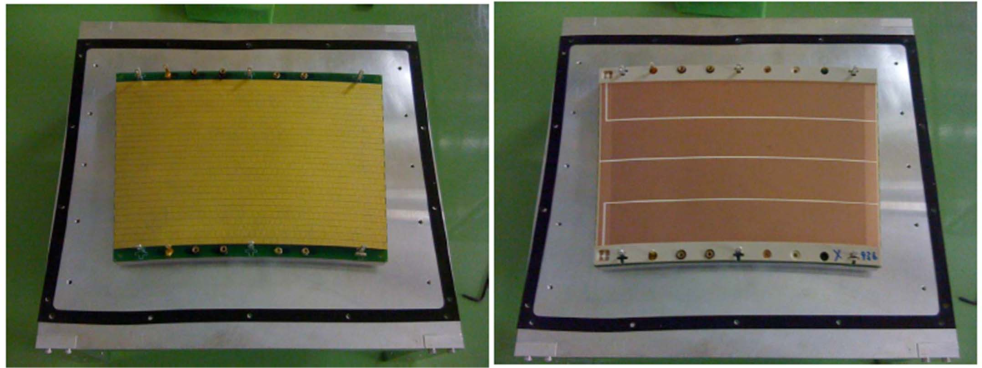
\includegraphics[width=0.9\textwidth]{Tracker/TPC_Bonn/plots/TPC-AG_Fig1asaingempicture}
  \caption{Asian GEM picture: left - anode pad plane; right - segmented cathode.}
  \label{fig_Fig1asiangempicture}
\end{figure}

Particles from the interaction point passing
between the modules may not be detected if they have very high momenta. Therefore, the Asian module foresees no frame along
the sides and extends the sensitive
area up to the edge of the backframe. To ensure a flat mounting of the GEMs, they are stretched on both the upper
and lower arcs (as seen in figure \ref{fig_Fig1asiangempicture}) which are made of a stiffer material:
GEMs with an insulator of \SI{100}{\micro\meter} Liquid Crystal Polymer (LCP)
covered with \SI{5}{\micro\meter} copper on both sides were produced by a company named SciEnergy.
The holes were
produced by \ce{CO2}-laser drilling after which they were carefully cleaned by dry etching to remove potentially
conductive residuals from the insides of the holes. The
hole pattern is identical to standard CERN GEMs. Because of the thicker material also higher gas gains per GEM
can be reached and a double GEM
structure is used and considered to be sufficient.
The two GEMs are mounted with an induction gap of \SI{2}{mm} and a transfer gap of \SI{3}{mm}.

The pad size is $1.2 \times \SI{5.4}{mm}$ and there are 28 pad rows with a total of 5152 pads.
From the beginning the use of an ion gate
(see subsection \ref{chap:TPC_sec:gating}) was envisaged and, thus, the level of the first GEM was designed
to be 1 cm below the nominal module height allowing for a later addition of the gate. To absorb the strength necessary
to stretch the GEMs and the gate, strong metal poles were implemented at the top and bottom arc.

\subsubsection{Recent Milestones}

All modules have been tested in the Large Prototype at DESY. The experience gained during all test beam periods as
well as the best transverse spatial resolution is described next. The testbeam measurements have used
the gas mixture of Ar-\ce{CF4}(3\%)-isobutane(2\%). The electric drift field was set in most cases to
E=\SI{230}{V/cm}, which is close to the maximum of the drift velocity, and alternatively to
E=\SI{130}{V/cm}, which is the minimum of the transverse diffusion.
The Asian modules were also measured using a laser system, in order to analyze the distortions.
The laser beam was scanned across the module, and the deviations were compared with calculations and are understood.

The Asian groups built three modules and made several test beam measurements at DESY (2009, 2010, 2012).
The first campaigns were dominated by very strong field distortions because of the mounting pins and the bare frames.
After introducing the field shaper, the distortions are comparable to the ones of other techniques used for modules.
The transverse spatial resolution is shown in figure \ref{fig_Fig2asiangemresolution}, where the measured spatial
resolution of a single row in the middle of a module can be seen.

\begin{figure}[!htb]
  \centering
  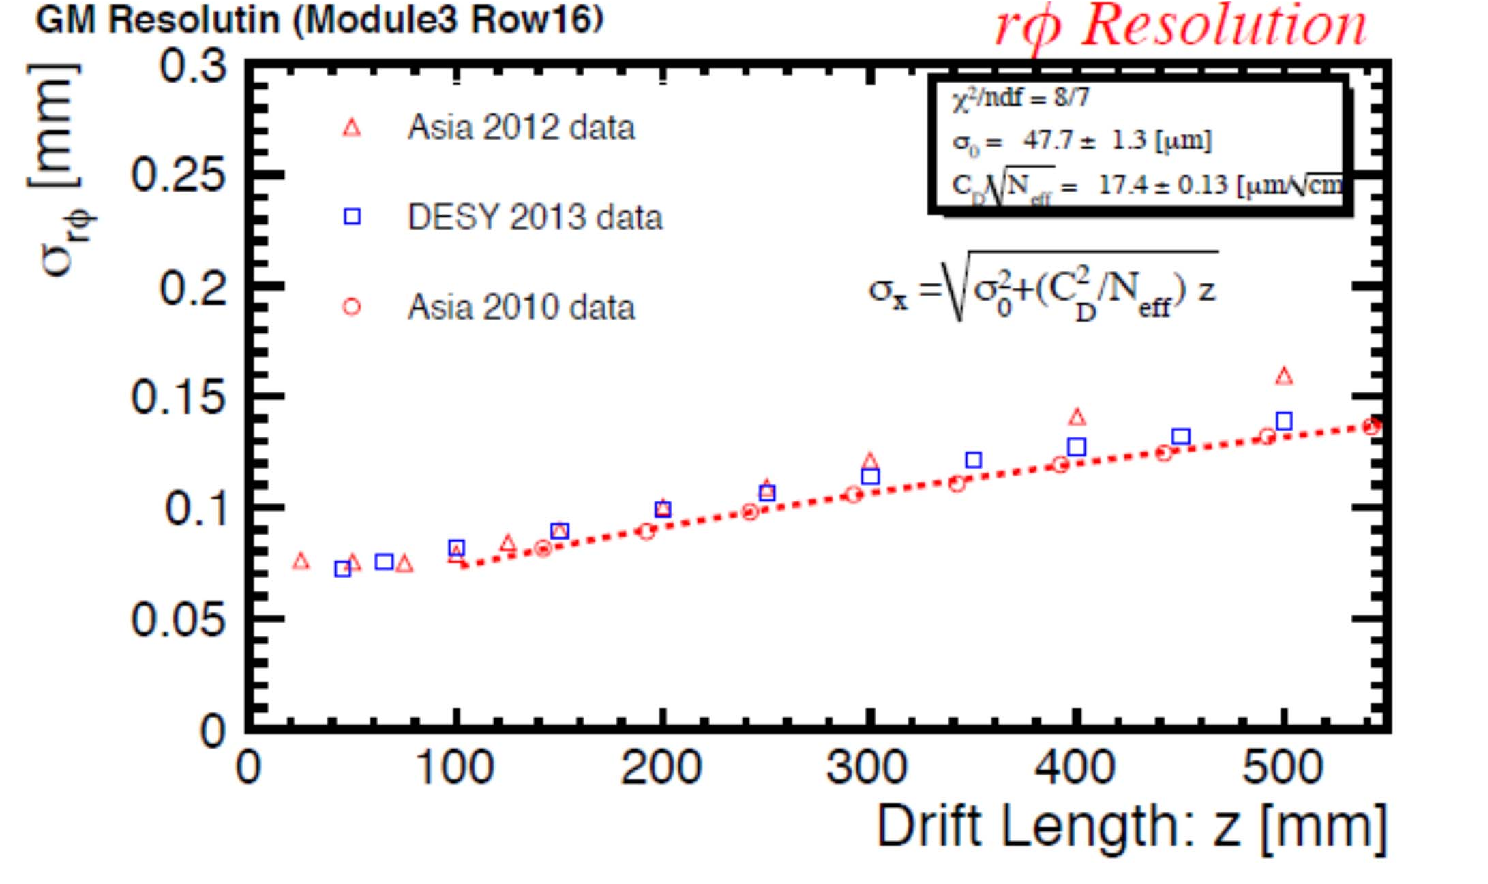
\includegraphics[width=0.9\textwidth]{Tracker/TPC_Bonn/plots/TPC-AG_Fig2asiangemresolution.pdf}
  \caption{Resolution measured for the Asian GEMs, and compared with a result for the DESY GEMs.}
  \label{fig_Fig2asiangemresolution}
\end{figure}

In this context an analytical formula was developed to predict the spatial resolution of a TPC. This formula includes
not only the effect of diffusion, angle,
noise and a finite pad-size, but also the influence of the electronics threshold, number of effective primary electrons,
the Polya-parameter of the gas
amplification, cross talk between pads and signal lines, charge loss because of attachment and the pad response function
are taken into account. All
these parameters can be varied and, if correctly chosen, describe well the measured data.

Finally, one other important observation was the HV micro-discharges on the Asian GEMs, with associated gain drops,
and investigations of this problem are summarized here.

To minimize the energy released in a discharge, the GEMs were segmented into four arcs, each with an area of
about $\SI{100}{cm^2}$ (figure \ref{fig_Fig1asiangempicture}, right).
Studies of the micro-discharges for the various types of GEMs were measured under a controlled environment.
The \SI{100}{\micro\meter} Asian GEMs discharged frequently, while the DESY \SI{50}{\micro\meter} GEMs (made by CERN) had little or no
discharges. For the \SI{50}{\micro\meter} GEMs, there is no significant difference of
the discharge rate between different types of GEMs. It is noteworthy that, at low gain, the \SI{100}{\micro\meter} GEMs
had a discharge rate which is almost the same as for the \SI{50}{\micro\meter} GEMs. The water content in the gas does not seem to
influence the
discharge rate, and long-term measurements are in progress.


\subsubsection{Future Plans}

In the future, it is planned to:\\
$\bullet$ understand better the reasons for the micro discharges and eliminate them, and \\
$\bullet$ construct a full scale Asian module with gate.

\subsection{Module type B, ``DESY Module''}
\label{chap:TPC_sec:DESY_gems}
Most recent update: 2016-03-28 \\
Contact person: Ties Behnke (email: ties.behnke@desy.de)\\

The goal of module type-B is a maximal coverage of the endplate with minimal dead area and a low material budget. It relies on thin ceramic frames to support the GEM foils on top of the readout plane \cite{Hallermann:2010zz,2012arXiv1202.6510D}, see figure \ref{fig:moduleAssembled}. The high stiffness of the ceramic frame allows the construction of very thin frames, which in turn minimize the dead areas of the module. With the current design only $\sim5\%$ of the active area is taken by the support structure and gaps between modules, the rest is sensitive area. The design of the system allows the simple stacking of GEM foils to build up compact, light weight self supporting multi-GEM modules. The development of this module type is led by DESY.

\begin{figure}[htb!]
\begin{subfigure}[b]{0.48\textwidth}
\includegraphics[width=\textwidth]{Tracker/TPC_Bonn/plots/TPC-DG_GemModule_Explosion.pdf}
\caption{}
\label{sfig:moduleExp}
\end{subfigure}
\hfill
\begin{subfigure}[b]{0.48\textwidth}
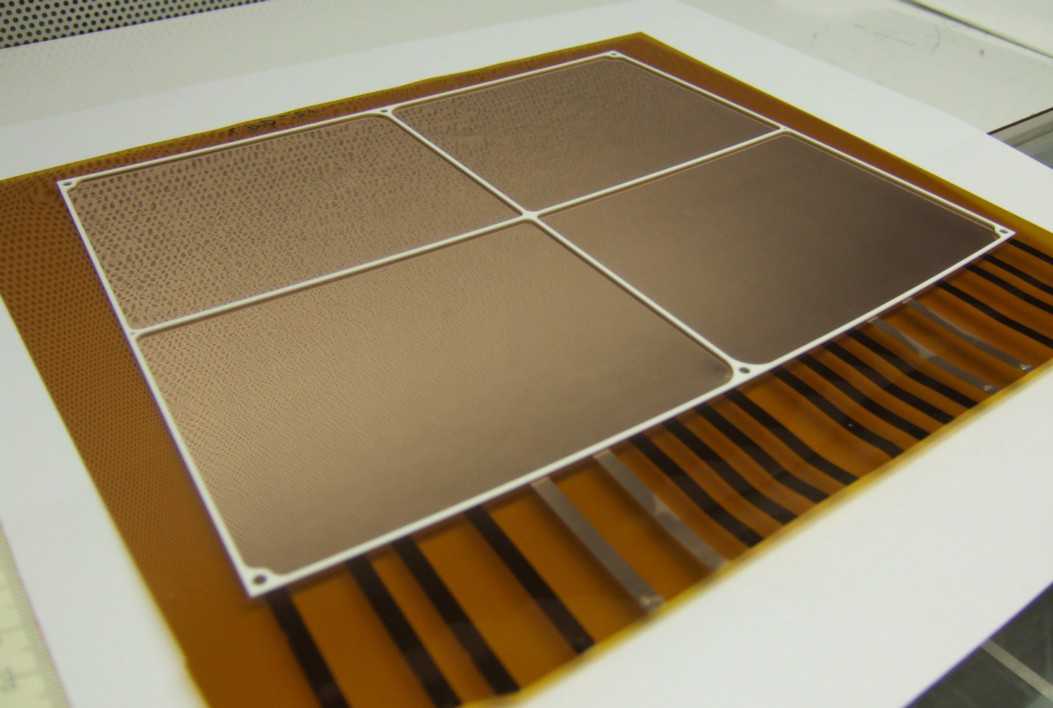
\includegraphics[width=\textwidth]{Tracker/TPC_Bonn/plots/TPC-DG_GemGrid.png}
\caption{}
\label{sfig:moduleGEM}
\end{subfigure}
\caption [Readout Module GEM]{\small \protect\subref{sfig:moduleExp})~Exploded view of one module showing the sequence of GEM foils and ceramic frames. \protect\subref{sfig:moduleGEM})~GEM foil with ceramic frame support used in the construction of the modules.}
\label{fig:moduleAssembled}
\end{figure}

\subsubsection{Recent Milestones}
Over the last years several test-beam campaigns took place and exposed three GEM based modules to test beam. Extensive data sets were collected with and without magnetic field, at different working points, and at different angles between the TPC and the beam.

For the first time the data taken were used in a global attempt to determine and correct field distortions. The Millepede-II \cite{Blobel20065,millepedeWiki} program was used to perform this global fit. First results indicate that distortions as large as several millimeters can be well corrected, see figure \ref{sfig:1Tdistort}. The resolution obtained both in $r\text{-}\varphi$ and $z$ behave as expected, and, if extrapolated to the running conditions at the ILC, meet the requirements, see figure \ref{sfig:resextrapol}.

\begin{figure}[htb!]
\begin{subfigure}[b]{0.48\textwidth}
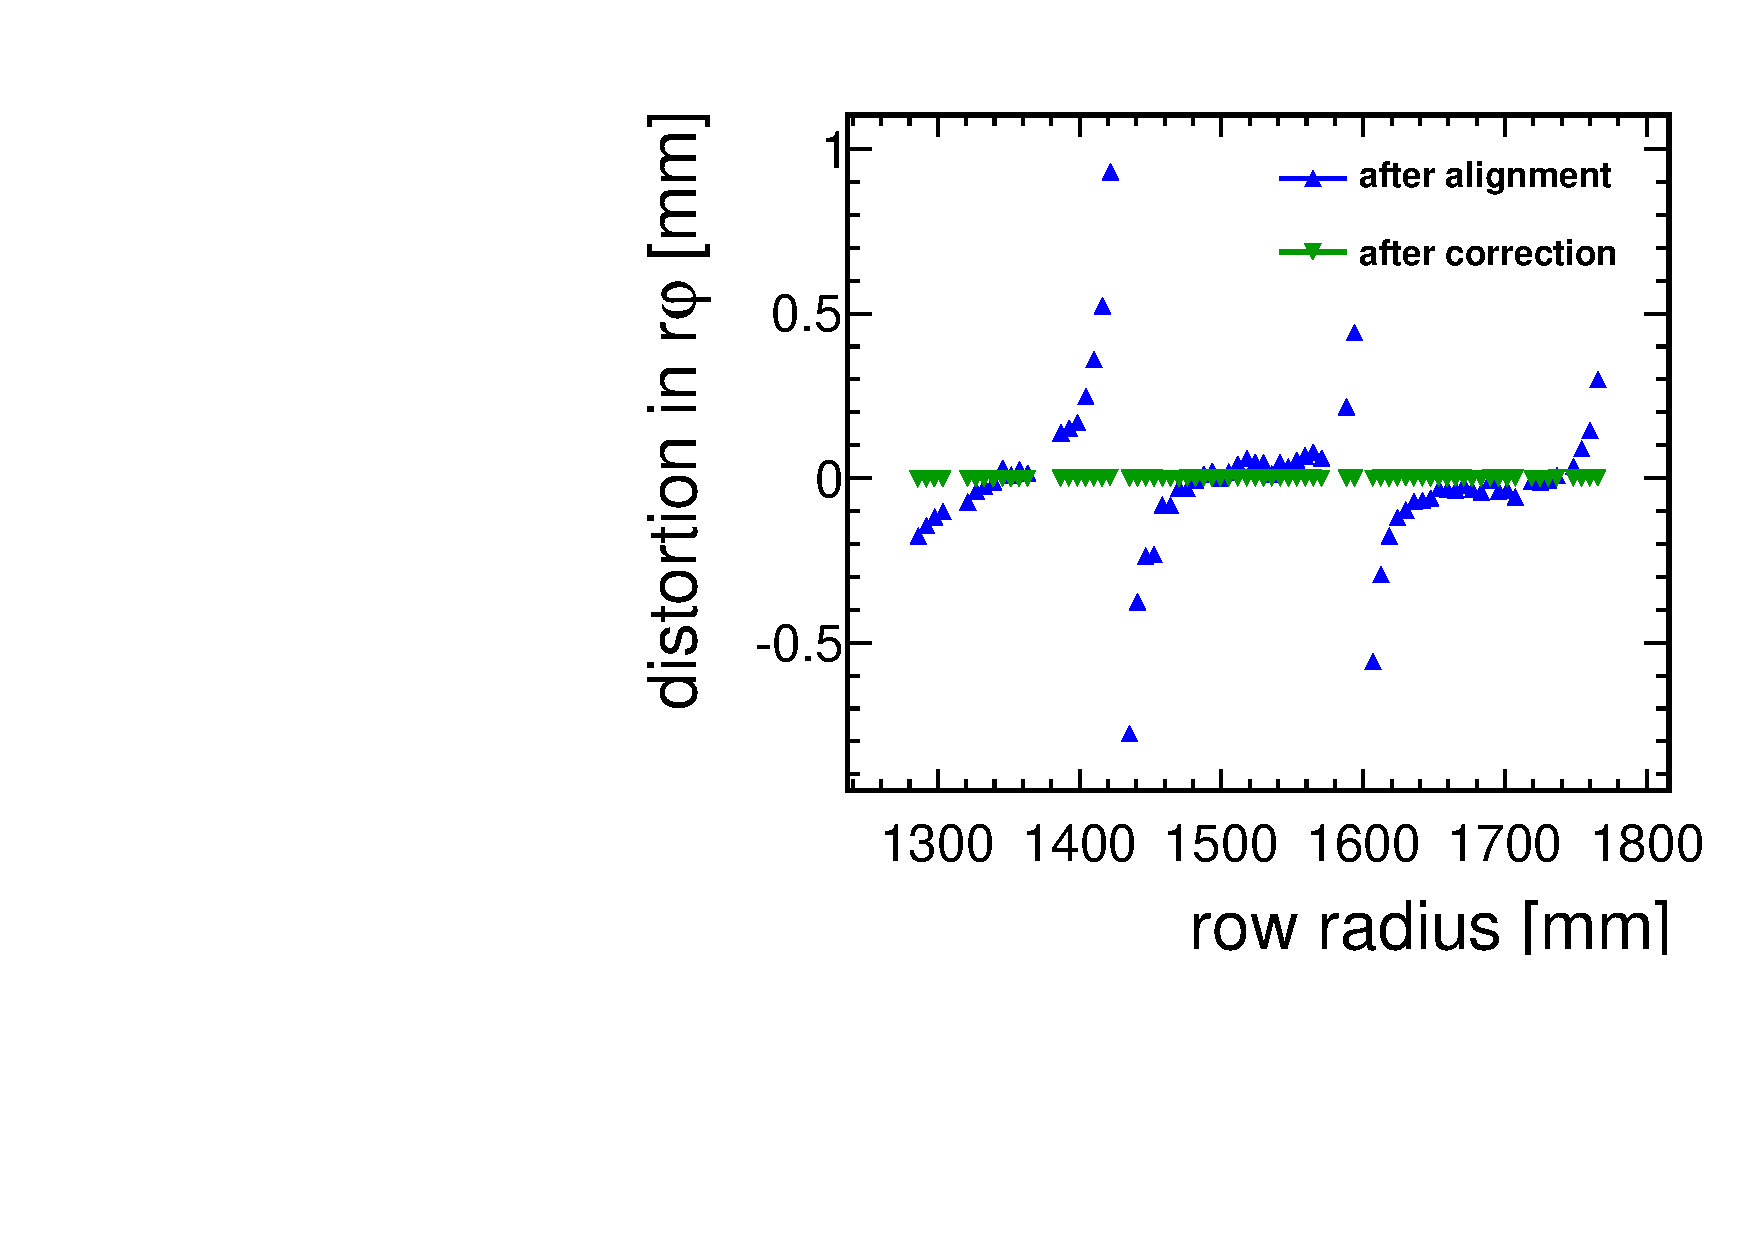
\includegraphics[width=\textwidth]{Tracker/TPC_Bonn/plots/TPC-DG_distortionAlignmentPaper1Tdistcor.pdf}
\caption{}
\label{sfig:1Tdistort}
\end{subfigure}
\begin{subfigure}[b]{0.48\textwidth}
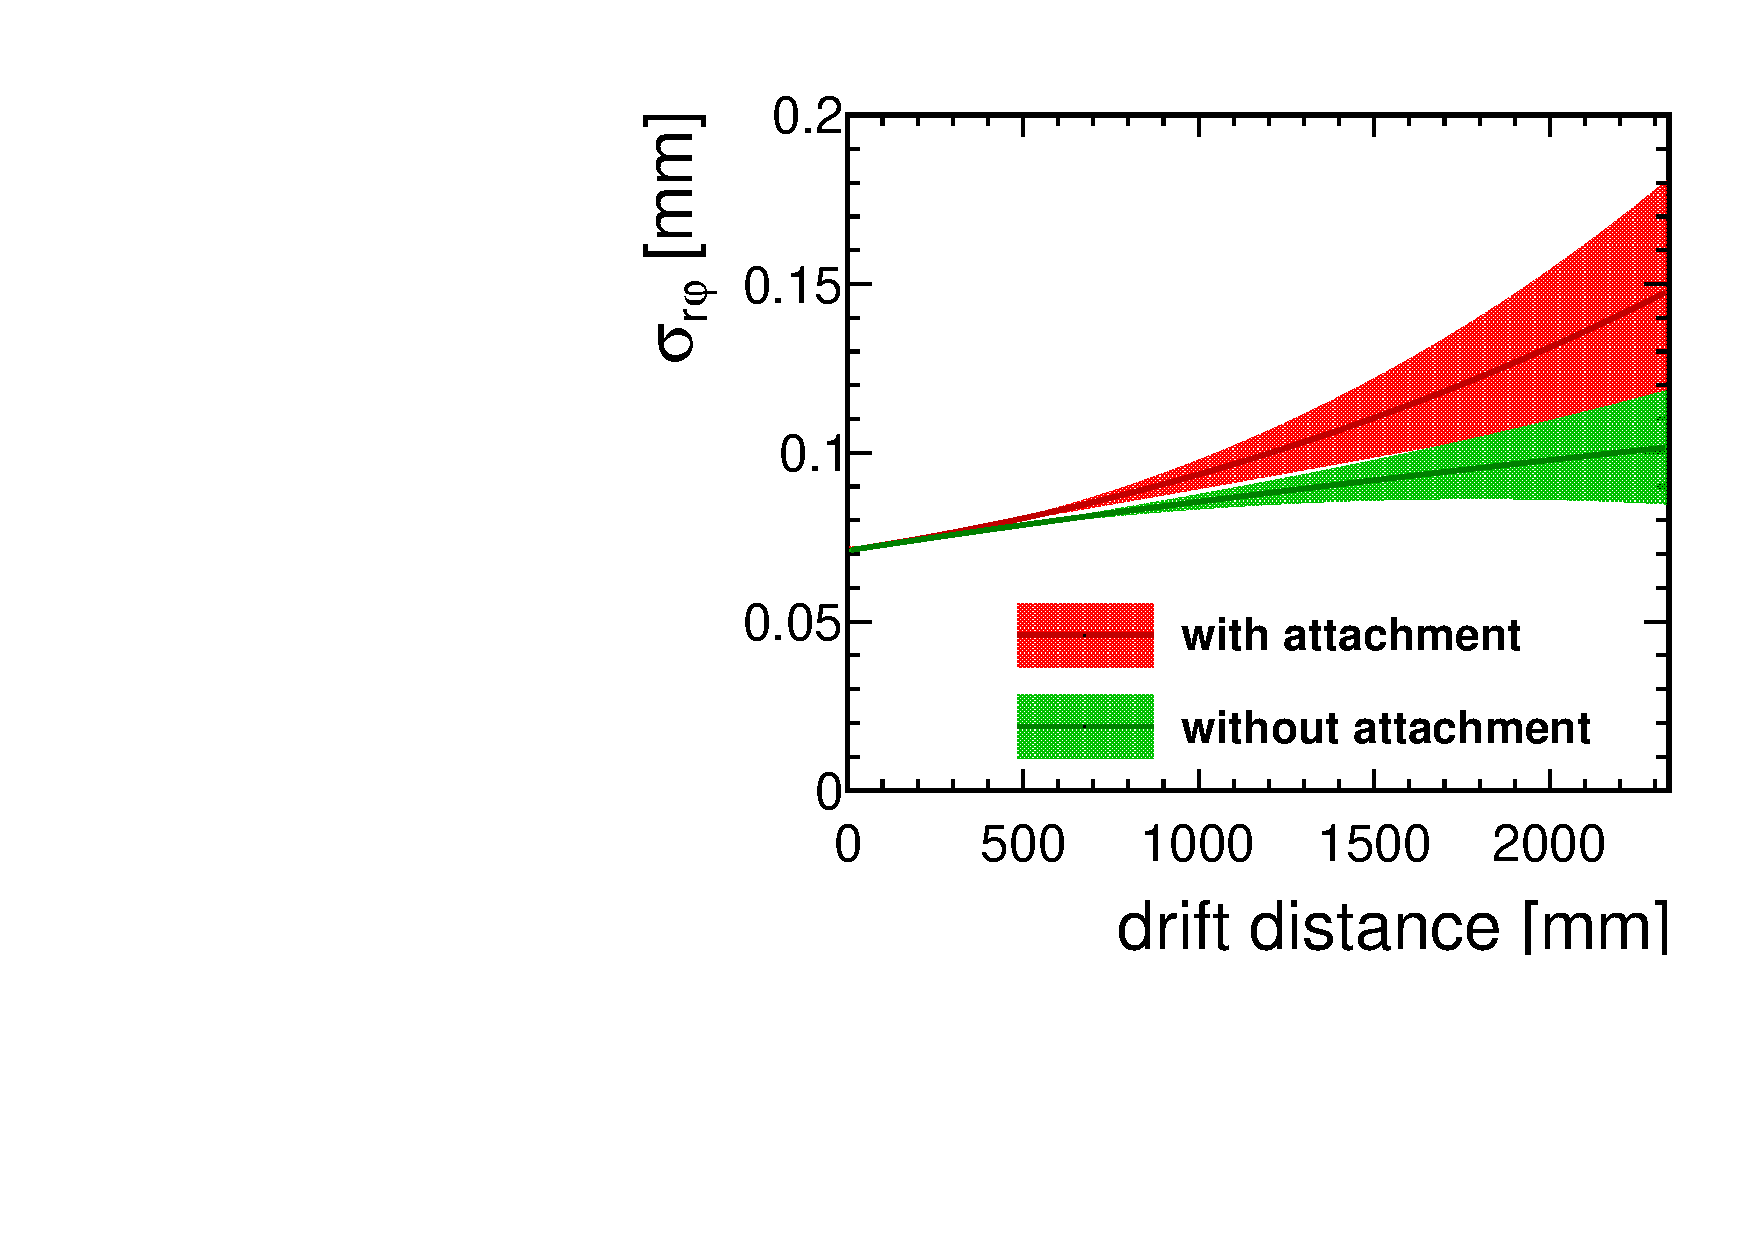
\includegraphics[width=\textwidth]{Tracker/TPC_Bonn/plots/TPC-DG_xyResolutionExtrapolated.pdf}
\caption{}
\label{sfig:resextrapol}
\end{subfigure}
\caption{\small \protect\subref{sfig:1Tdistort})~Alignment and distortion correction: mean hit position in $r\varphi$ with respect to the track position at \SI{1}{T} versus pad row radius. In blue after alignment correction, in green after distortion correction. \protect\subref{sfig:resextrapol})~Point resolution: extrapolation to a magnetic field of \SI{3.5}{T} based on parameters measured with the Large TPC Prototype at \SI{1.0}{T}. Plotted over the full ILD TPC drift length of \SI{2.35}{m} including 1 \sigma error bands. In red with the measured attachment rate, in green without any attachment.}
\label{fig:align1Tdistort}
\end{figure}

The field homogeneity was in addition studied in dedicated laser runs \cite{Zenker:2014qra}. A UV laser illuminates the cathode plane in the TPC, on which dots are placed made from a material with a small work function. The laser light extracts electrons at the position of the dots. These electrons are then drifted towards the anode, and are measured. From the dislocations of the dots relative to the known position on the cathode, the integrated effect of field distortions in the TPC volume can be measured.

Extensive simulations of the behavior of the GEM foils in case of electrical breakdown were performed. They showed that a strong coupling exists between the different regions of the GEM foil. In some cases these couplings can trigger secondary trips in the module, which in rare cases can damage the GEM. A protection circuit is currently under development and will be tested in the near future.

%\subsubsection{Engineering Challenges}
\subsubsection{Future Plans}

By now two generations of these modules have been developed and successfully tested. The main issues which are going to be addressed in the next 1-2 years are
\begin{itemize}
\item re-optimisation of the support structure for maximum mechanical strength and minimal interference with the readout
\item development of a protection scheme which will ensure safe operation of the module even in case of high-voltage trips.
\item optimization of the field-shaping integrated into the module, to minimize field distortions close to the module and at module boundaries.
\item integration of a GEM based gate on top of the current amplification structure, based on the recent developments at KEK.
\end{itemize}
It is planned that within the next six months a third generation module design will be developed and several modules built which will address these challenges.

\subsubsection{Engineering Challenges}
%The GEM based modules face rather similar engineering challenges. Among the most important one is the optimisation of the overall mechanical structure, to provide adequate mechanical strength, without introducing excess dead material.
A detailed study is ongoing to understand and quantify the mechanical behavior of the ceramic frame GEM system. Bending tests have been performed, and compared to simulations. The interference between the mechanical properties and the electrical properties are studied. Measurements of the flatness of the module are being done, and will provide input for the next design iteration.
The fabrication of the ceramic frames which is currently done by laser cutting from solid sheets of ceramic will be studied. Possible alternatives are 3D printing of the frames. Improvements in the laser cutting technology might allow thinner frames, without loosing stiffness.

Another open question is the distribution of the high voltage from the endplate to the different GEM layers. The current solution is rather labour intensive, and relies heavily on the skills of the person doing this connection. Faults are difficult to find, and even more difficult to repair. Here new solutions are being sought, which are more easily to produce, more reliable, and will give better high voltage security. Connected to this are the protection schemes against accidental high voltage discharges, which are still not perfect.

As discussed in section \ref{chap:TPC_sec:gating}, a gating GEM will be implemented as part of the amplification scheme. This gating GEM needs to be mechanically integrated into the module.

Currently a gap of about \SI{2}{mm} exists between neighboring modules. This gap introduces significant field distortions \cite{Zenker:2014qra}. They are partially compensated by a field shaping strip on the outside of each module. However a better and more robust solution would be to further minimize the gap between modules. Doing so will need improvements of the high voltage distribution, as discussed above, but also of the overall mechanical integration of the modules into the endplate.

%\subsection{Applications Outside of Linear Colliders}


\section{Resistive Micromegas}
\label{chap:TPC_sec:micromegas}
Most recent update: 2016-03-28\\
Contact person: Paul Colas (email: paul.colas@cea.fr)\\

\subsection{Introduction}
First Micromegas prototypes were built with a micro-mesh stretched on a frame, and kept on top of
a segmented anode at a fixed distance of \SI{50}{\micro m}. The gap is defined by spacers manufactured
by photo-lithographic techniques. Early tests confirmed that, due to ``hodoscope effect'' a resolution
down to \SI{100}{\micro m} could not be reached \cite{Arogancia:2007pt}. This triggered studies with charge spreading
developed at Carleton University~\cite{Dixit:2003qg}.
The first resistive material was an AlSi CERMET deposited on a Mylar foil and glued at
\SI{90}{\degreeCelsius} with layer of melting polymer~\cite{2007NIMPA.581..254D}. Later on, a more robust resistive material was
used: the Dupont-de-Nemours Carbon-loaded Kapton. Novel way to manufacture the Micromegas detector
were perfected by the Saclay group in partnership with CERN.


\subsection{Recent Milestones}
From 2008 onward, tests with resistive Micromegas were performed in the Large Prototype. From 2008 to 2010
a single module sitting in the middle of the endplate was tested, with dummy modules all around. The 1726 pads, each about \SI{3}{mm} wide
and \SI{7}{mm} long,
were arranged in 24 lines and 72 radial columns, with 2 pads sacrificed to bring the high voltage to the mesh
through the PCB. The standard electronics from the T2K/ND280 neutrino experiment based on the AFTER chip
was used, connected through 20 to \SI{40}{cm} long flat cables~\cite{6418152}.
To minimize the dead area, the so-called ``bulk'' \cite{Giomataris:2004aa} process was used to fix the
mesh on the PCB: in this process a stainless-steal mesh is held by polyimide pillars sandwiching the mesh, melt together
through the mesh. This makes a robust and dust-proof detector, with only \SI{2}
{mm} taken by a grounding ring at the periphery of the module. This ring is used to fix the potential of the resistive anode all around.

Data taken in this 1-module configuration allowed several resistive coatings to be tested. Resistive pastes were discarded, as
their electrical properties were not uniform enough and lead to distortions on the hit position. Carbon-loaded Kapton gave
very good results, with a resolution down to \SI{70}{\micro m} at zero drift distance.

Starting in 2011, a completely new integration of the electronics has been carried out to allow the simultaneous operation
of 7 modules. Naked chips were directly wire-bonded on cards. All the protection of the electronics was removed, this functionality
being fulfilled by the resistive coating. The ADC was moved from the front-end to a mezzanine card, all the electronics fitted just behind the module.
At the same time the noise and the power consumption were lowered by 25\%. To connect a module with 1726 channels, only
3 cables need to be connected: a High Voltage cable for the gaseous amplification, a low voltage cable to supply the electronics,
and an optical fiber to transport the data and the command parameters to the mezzanine card.
The production of 9 modules (including 2 spares) and their electronics followed a quasi-industrial scheme.

Data with 7 modules were taken in 2014 and 2015, allowing new topics to be addressed, as module alignment and distortions.
ExB effect induces distortions for tracks reconstructed near the module boundary causing
shifts of almost 1 mm for pad hits located at the extremity of the module.


This is
in agreement with the simulations carried out in the Kolkata group and which can be corrected down to \SI{20}{\micro m}.

In 2014 and 2015, a two-phase \ce{CO2} cooling was provided to the 7 Micromegas modules. The two-phase coolant, under a pressure of \SI{50}{bar}, circulates at a temperature close to the ambient.
It consists presently of a serpentine running on the back of the modules, in good thermal contact with Aluminum heat sinks, themselves in contact with the chips. The pipe diameter is less than a millimeter, giving a moderate contribution to the material budget. The unit
which provides the pressurized \ce{CO2} was funded by KEK and designed by a Nikhef-CERN collaboration.
An efficient cooling was observed for more than 80 hours continuously.

In 2015, two new modules were inserted on the endplate. The resistive material of the new
modules was Diamond-Like Carbon obtained by sputtering on a Kapton foil.
This gives a very robust resistive anode, and the procurement of this material, made in Japan, is more reliable
than the Dupont Carbon-loaded Kapton. These two modules showed identical performance as the other modules.

\subsection{Engineering Challenges}
Special care will have to be given to the design of the edge of the modules, to have a uniform potential on the exposed surface of the pad while the boarders of the modules must be grounded.

The adaptation of a gating device at a few cm from the end-plate, or integrated to each module, is a
difficult engineering challenge if a minimal degradation of the performances is to be obtained.


\subsection{Future Plans}
The time structure of the beams will produce positive ion backflow disks moving slowly (at a few \SI{1}{m/s}) towards the cathode. To experimentally address the question of the effect of these ion disks on the drifting electrons, it is projected to produce such
ions by casting UV light to the cathode for a ms every \SI{100}{ms} or so, while observing distortions on cosmic-ray or beam tracks.
Last but not least, the momentum resolution should be evaluated with long tracks from a particle beam, which requires a silicon
tracker inside the magnet to measure precisely the track position and momentum. For the cooling, further integration work is needed, using micro-channels in the detector board and new material choices for the sink.

In summary, the Micromegas TPC R\&D successfully underwent its proof-of-principle phase and the main integration questions are now addressed. They now request targeted design to progress, thus specific project funding.

\section{Pixelized Readout}
\label{chap:TPC_sec:pixels}
Most recent update: 2018-11-01 \\
Contact person: Klaus Desch (email: desch@physik.uni-bonn.de)\\

\subsection{Introduction}
To make the most of the fine pitches of the Micropattern Gaseous Detectors the
readout structure should be adapted to the same feature size. Therefore,
readout ASICs of silicon pixel detectors such as the Timepix ASIC
\cite{Llopart2007485, Llopart2008106} can be placed directly below the gas amplification
stage. In this setup, the bump bond pads normally used to connect the readout
chip to the Si-sensor are used as charge collection pads. In some studies a
triple GEM was used as a gas amplification stage \cite{Bamberger:2006xp, 6359808},
while in others a Micromegas has been built
directly on the ASIC \cite{4526754}. The latter detector type is 
 called GridPix and is produced by using a post-processing technique, which
 guarantees a high quality grid perfectly aligned with the readout pixels. This
 alignment ensures that the complete charge avalanche initiated by a primary
 electron is collected on one pixel. Because of the high signal-to-noise
 ratio both tracking and dE/dx measurement benefit from distinguishing and
 detecting single primary electrons with a high efficiency. This type of
 detector was pioneered by Nikhef/University of Twente (NL). The University
 of Bonn has modified the 
 production process together with the Fraunhofer Institut IZM so that a
 wafer-based production of GridPix detectors is standard by now
 \cite{Koppert2013245}. First tests were done with both
 gas amplification stages by using single ASICs with an active area of about \SI{2}{\centi\meter\squared}. The detectors were operated in laboratories at Nikhef, Saclay, Bonn,
 Freiburg and Siegen to test the working principle. It could be demonstrated
 that the transverse spatial resolution of the reconstructed primary electrons
 was close to the expected diffusion limit of single electrons. 

 \subsection{Recent Milestones}
At the University of Siegen new types of GEMs are being tested in combination
with the Timepix ASIC: GEMs with a carbon coating on the copper electrodes and
GEMs with a ceramic insulator. Both types are tested in a prototype setup and
compared to standard CERN GEMs.

At Nikhef, Saclay and Bonn several projects were carried out to demonstrate
multi-module operation and large area coverage of modules with GridPix
detectors. The new GridPixes were also assembled in 8
GridPix modules for the Large Prototype detector at DESY. Successful test beam
campaigns were performed in 2010 with a single module and in 2013 and 2014 
with two modules \cite{1748-0221-9-01-C01033}. Up to three LP modules
with a total of 160 GridPixes were operated in a test beam. The central module was equipped with 96
GridPixes and the two outer modules had 32 GridPixes arranged to maximize the
lever arm. 
\begin{figure}[!t]
  \centering
  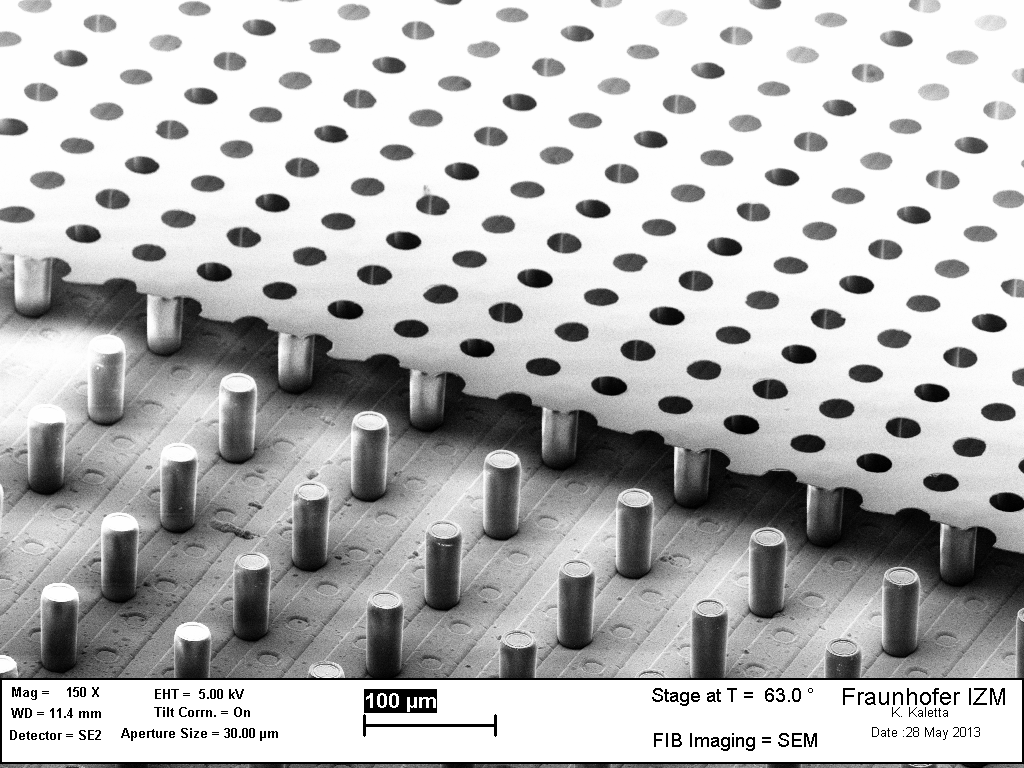
\includegraphics[width=0.45\textwidth]{Tracker/TPC_Bonn/plots/TPC_pixels_GridPix.png}
  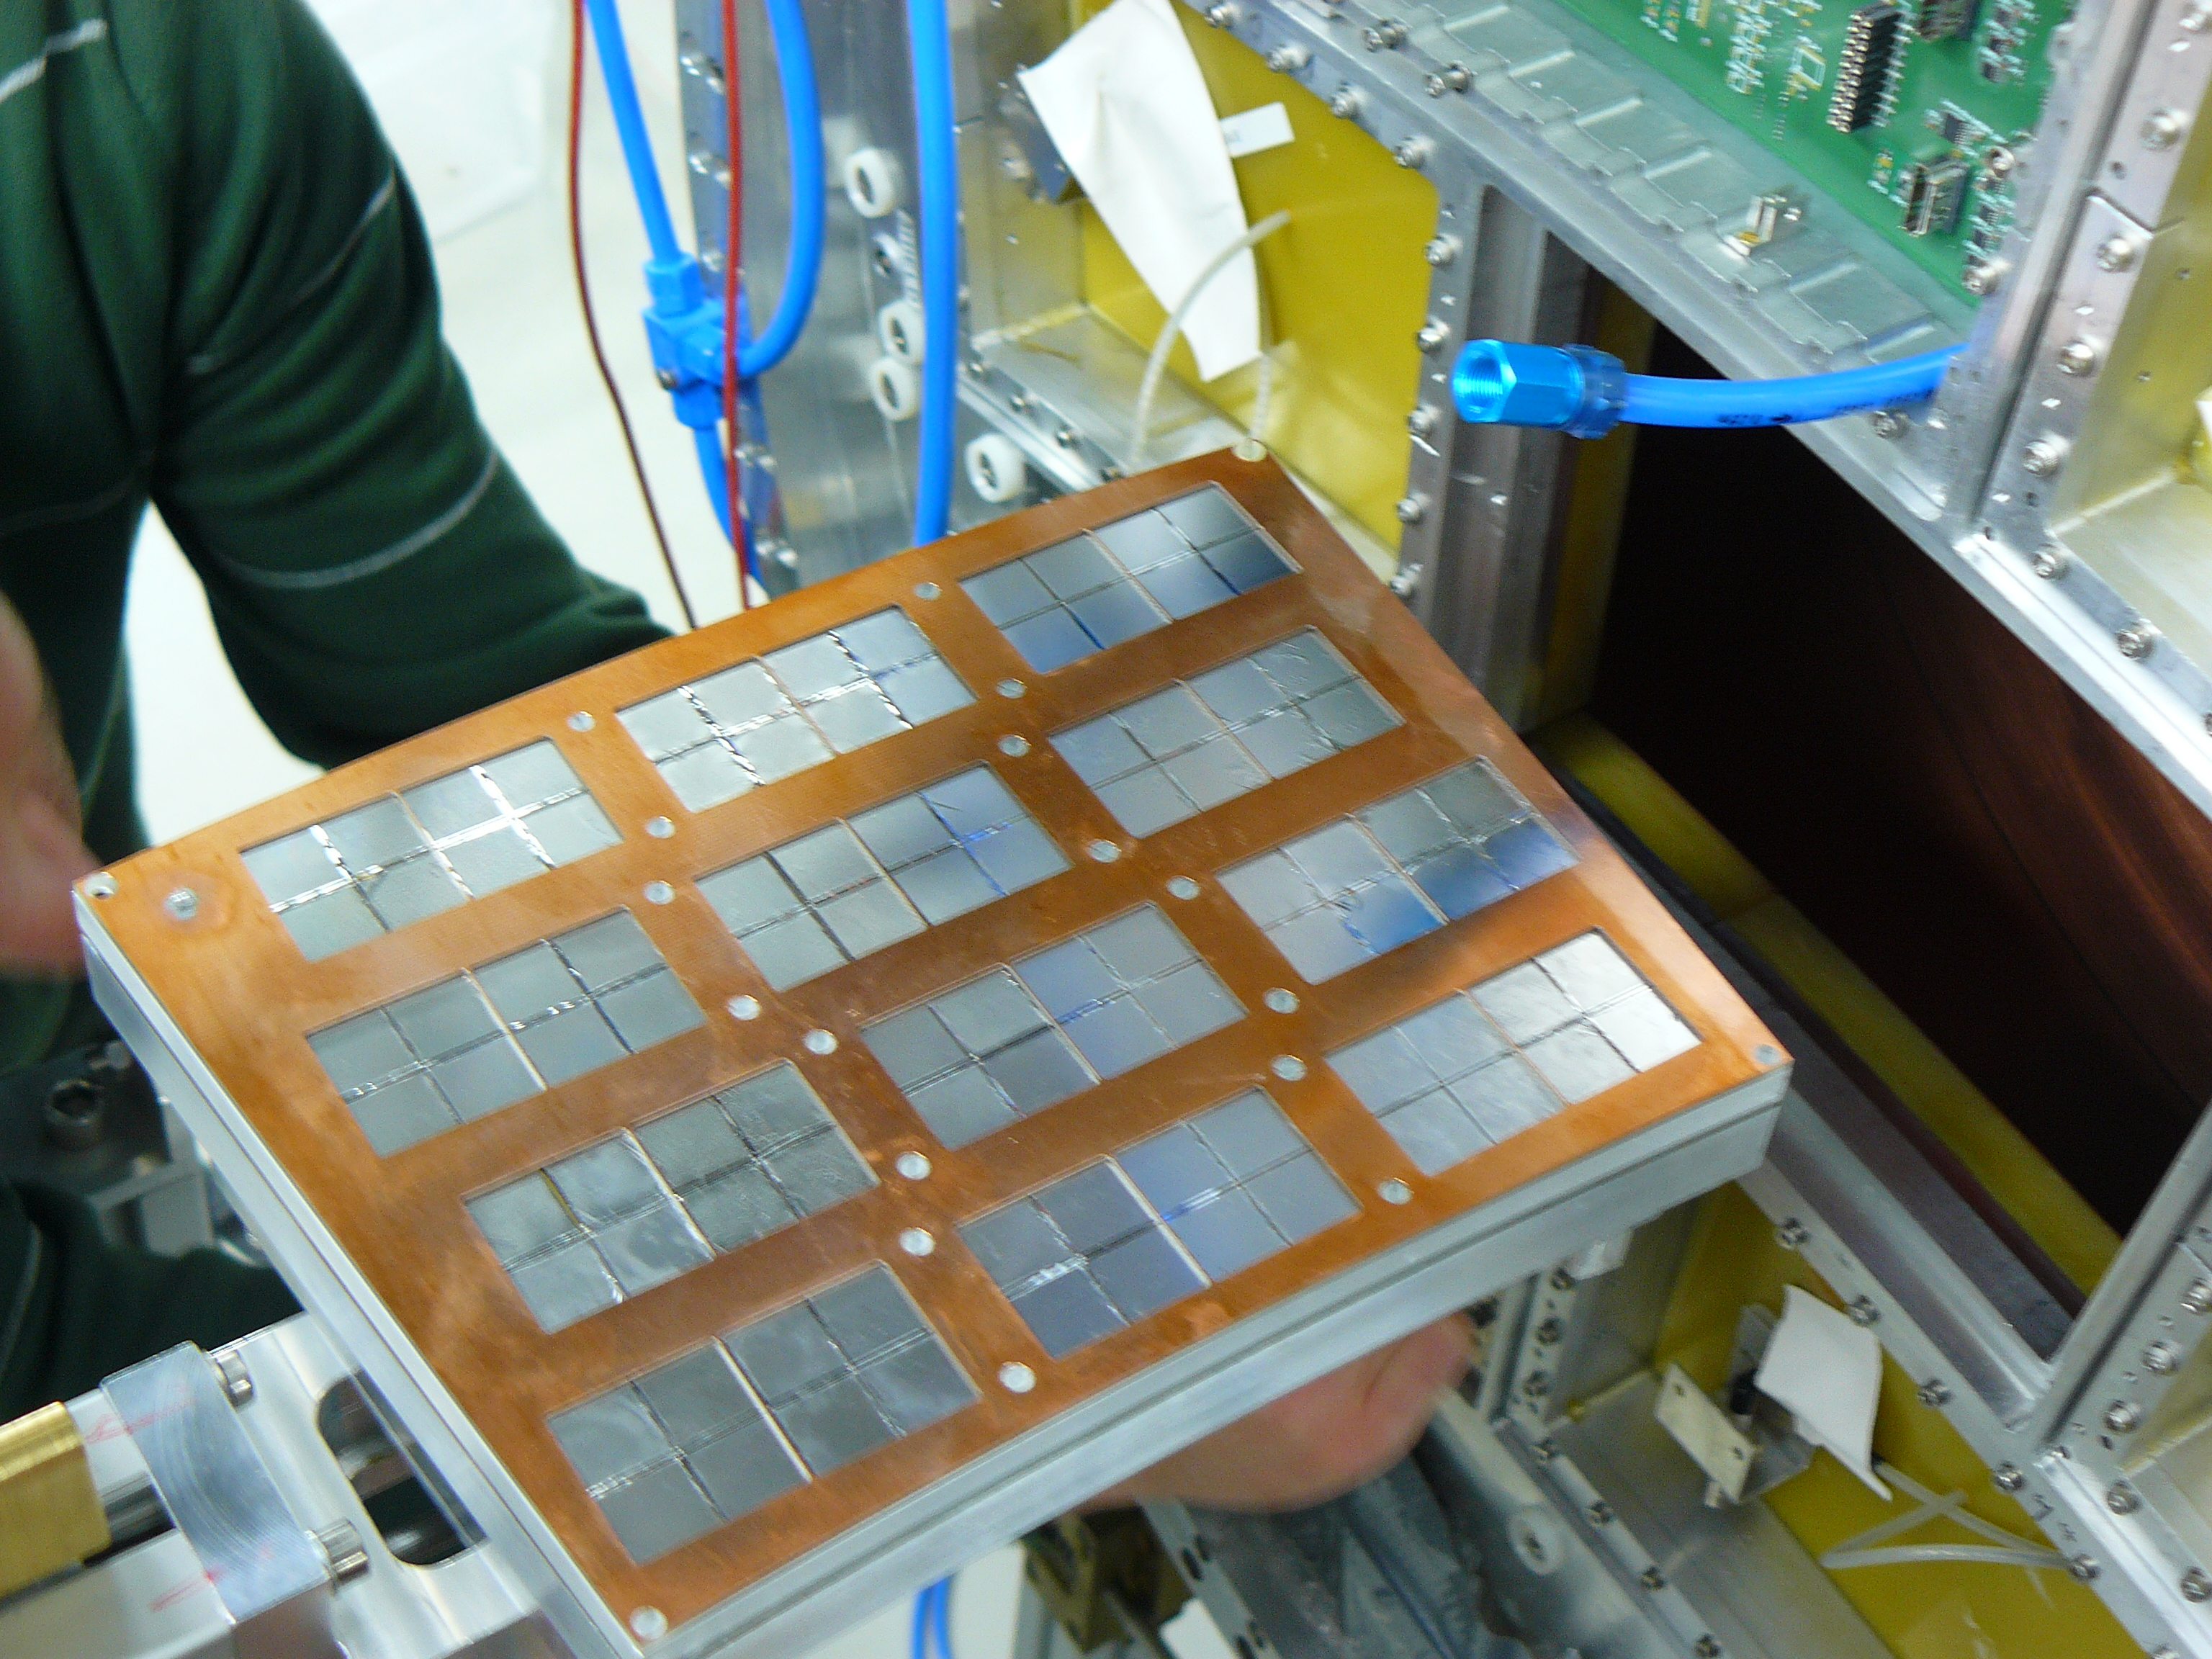
\includegraphics[width=0.45\textwidth]{Tracker/TPC_Bonn/plots/TPC_pixel_complete_module.png}
  \caption{Left: SEM picture of an InGrid detector with a partially removed
    grid, right: Fully equipped LP module with 96 GridPix detectors is being
    mounted in the LP.}
  \label{fig_TPC_pixels_1}
\end{figure}

This setup served as a demonstrator that larger areas ($\sim$\SI{400}{\centi\meter\squared}) could be produced and operated. It was tested in the Large Prototype in March/April of 2015 and operated for more than one week permanently in the
test beam. A total of about 200 runs with more than 1.5 million events were recorded \cite{7889045}.

\begin{figure}[!t]
  \centering
  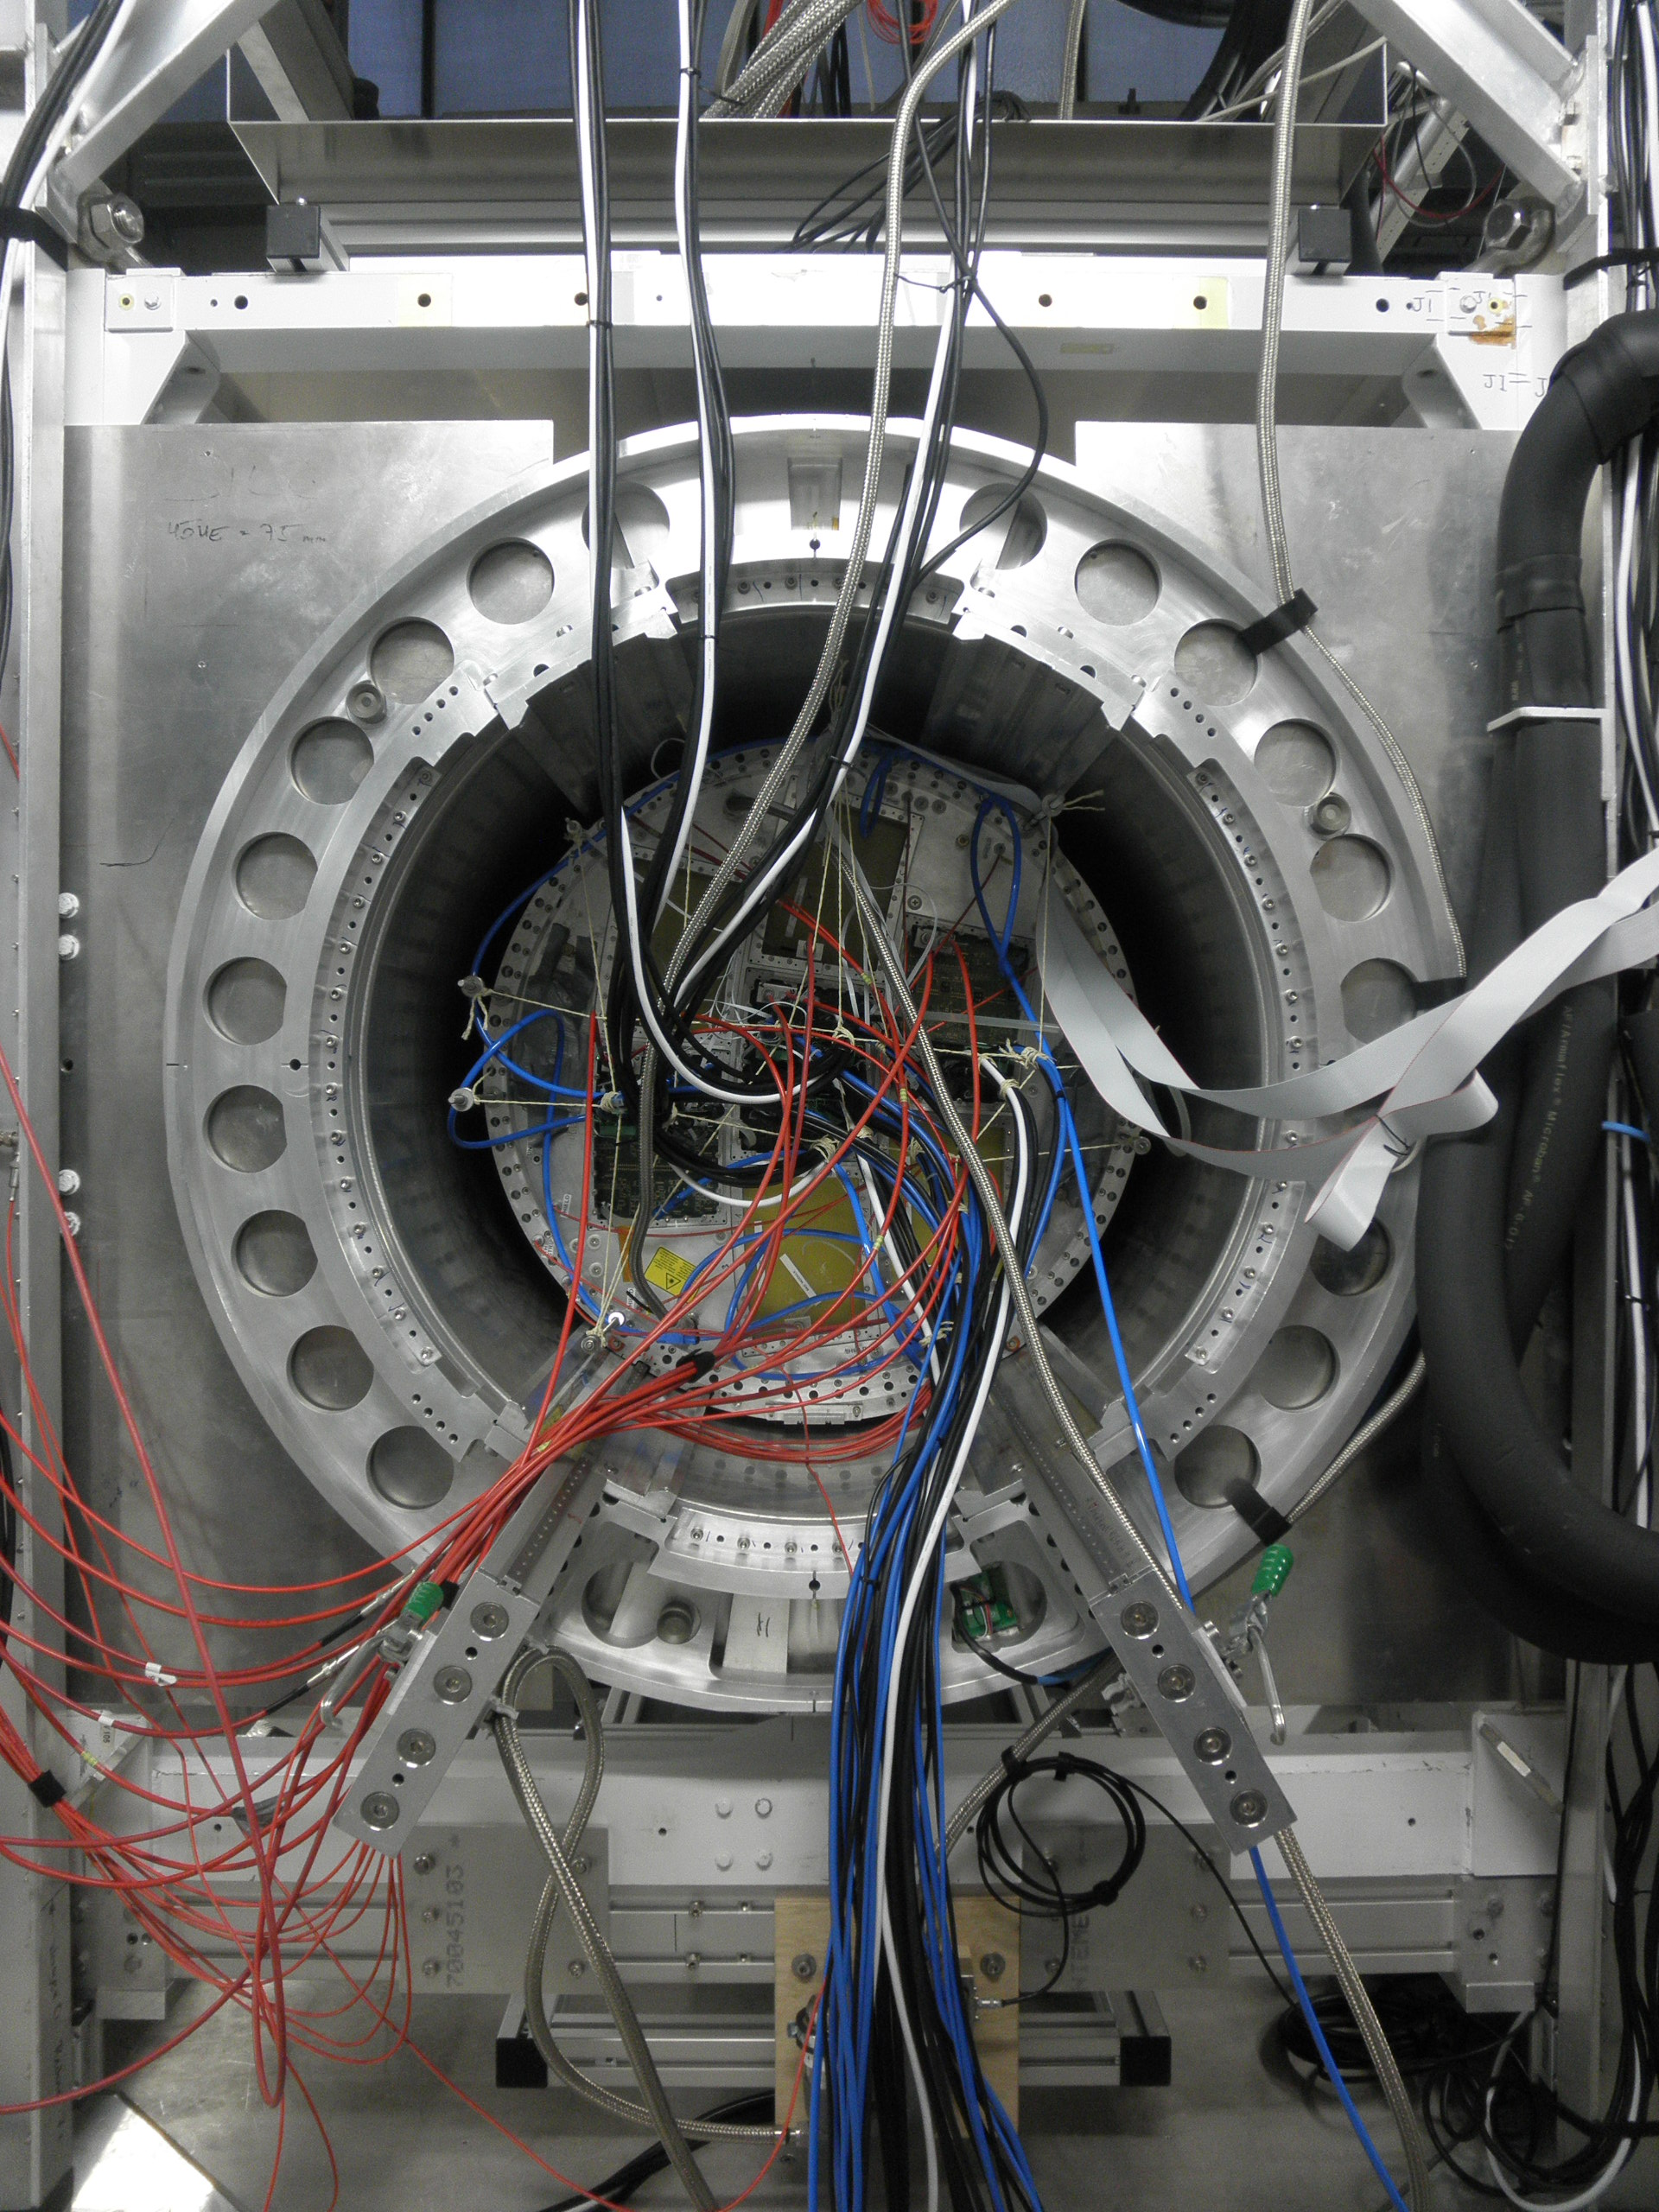
\includegraphics[width=0.28\textwidth]{Tracker/TPC_Bonn/plots/TPC_pixels_LP_GridPixes.png}
  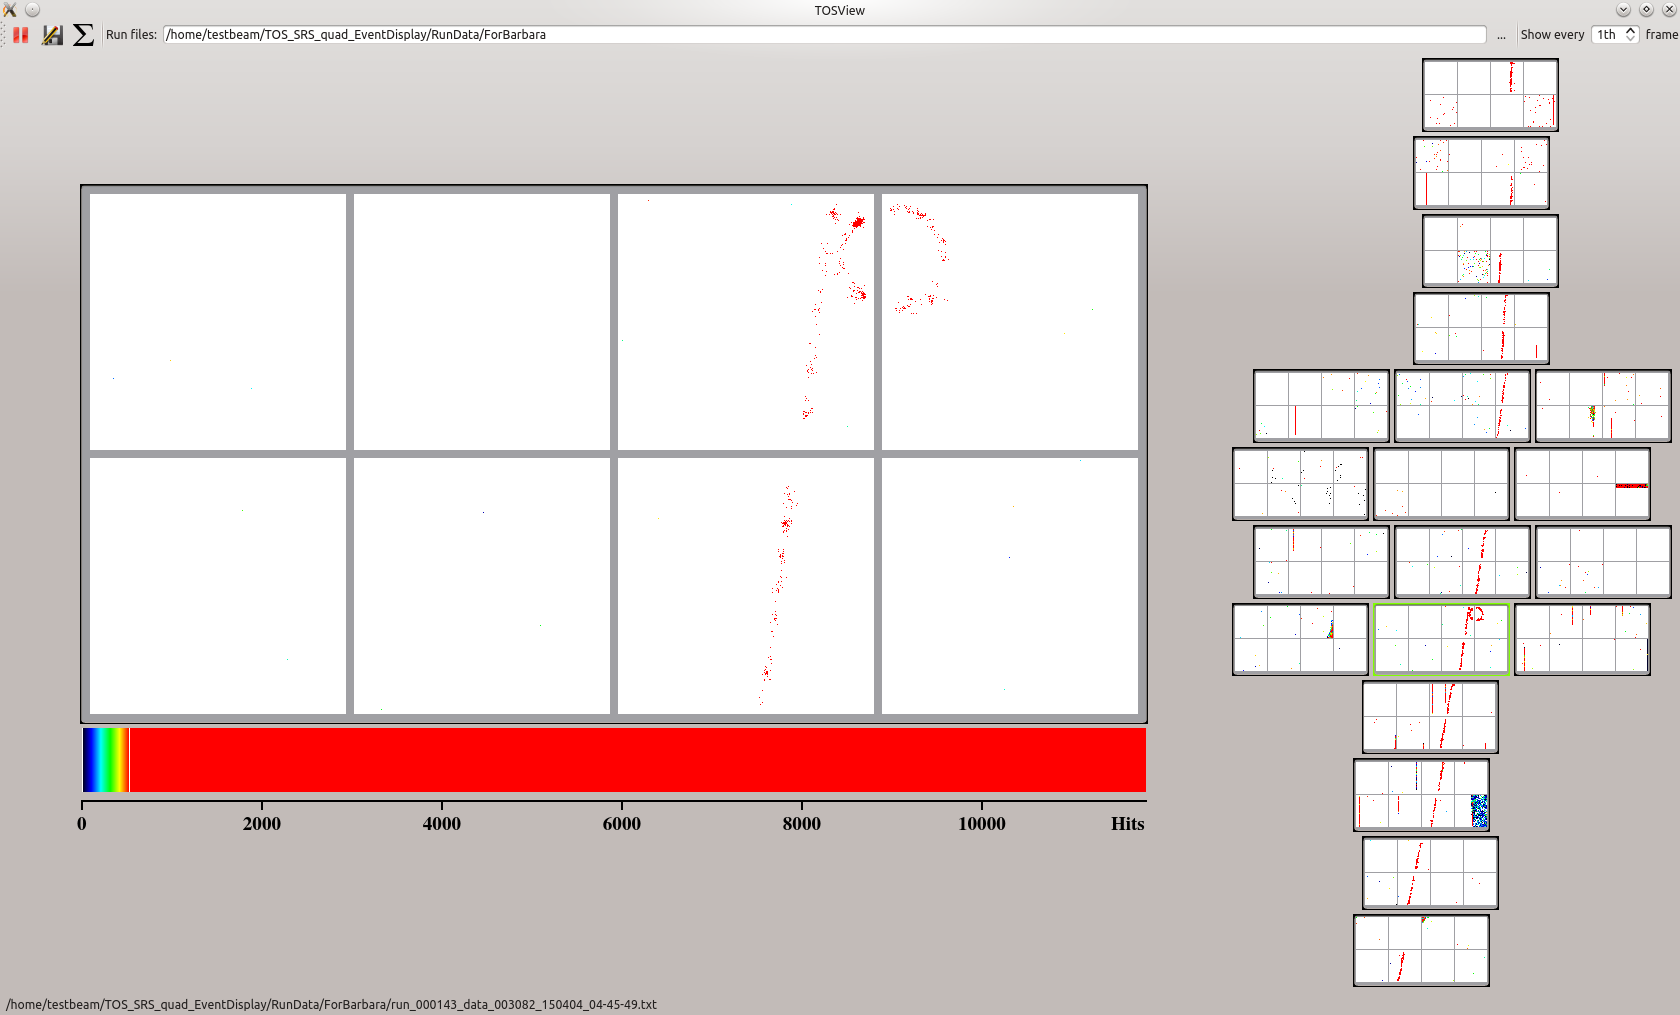
\includegraphics[width=0.62\textwidth]{Tracker/TPC_Bonn/plots/TPC_pixels_event.png}
  \caption{Left: Three modules with 160 GridPix detector mounted on the Large
    Prototype, right: Online event display of a 2 track event recorded with
    160 GridPixes.}
  \label{fig_TPC_pixels_2}
\end{figure}

Nikhef and Bonn have also taken part in designing a successor ASIC of
the currently used Timepix. The new Timepix-3 features several improvements,
which promise a much better performance. In particular it is multi-hit capable,
can record both time and charge of each signal, has a much faster
digitization frequency (\SI{640}{\mega\hertz}) and can be read out  quasi continuously.
Also, the grid design was revised increasing the active area to 97.7\% of the pixel area. First Timepix-3-based GridPix detectors have been built and tested. A testbeam campaign was conducted in July 2017 at the ELSA accelerator in Bonn and a single GridPix detector was exposed to an \SI{2.5}{GeV} electron beam \cite{Ligtenberg:2018sjs}. The performance clearly surpassed the one of Timepix-based GridPixes. In particular the longitudinal spatial resolution could be improved by over one order of magnitude. 
As a next step, in 2018 a quad consisting of four GridPix detector was constructed and
tested~\cite{Ligtenberg:2020ofy}. Special attention was given to the mechanical and electrical design of the
guard structure to maximize coverage and minimize distortions. The distortions in the
precision plane stay below the 13 microns and meet the design specifications of a TPC at a
linear collider. A module consisting of 8 Quads has been constructed and will be tested in
2020.

\subsection{Engineering Challenges}
The production of modules with large area coverage requires to solve four
major technical challenges: 
\begin{enumerate}
  \item The production of a large number of GridPixes with sufficiently good
quality. This has been addressed by the new production method, which is based
on complete wafers. The process was developed in collaboration with the
Fraunhofer Institute IZM at Berlin and yields up to 428 GridPixes per batch (4 wafers). 
\item In particular commercial readout systems are not easily scalable to a large number of chips. This is why Bonn has developed a cheap and easily expandable system based on the Scalable Readout System (SRS) of the RD51 collaboration.
Nikhef developed (partially funded by the AIDA FP7 project) the SPIDR fast readout system for Timepix-3 ASICs \cite{1748-0221-10-12-C12028}.
\item Current water cooling has to be replaced by 2-phase \ce{CO2} cooling.
\item In order to overcome systematic limitations of track reconstruction, field
  distortions caused by tilted chips and only partially covered ground
  potentials need to be mitigated.
\item In order to reduce the ion back flow a gating grid (as discussed below in section~\ref{chap:TPC_sec:gating}) can
be installed. For a GridPix a solution based on a double grid - with a same hole pattern - is possible.
This will reduce the ion backflow continuously(, as e.g. needed for high luminosity Z running
at circular a machine). Both the gating grid and the double grid solution need further
studies and tests.

\end{enumerate}

\subsection{Future Plans}
Currently the main focus is on the analysis of the test beam data. The
challenge of finding and fitting tracks with several thousand hits is quite
different from the standard pad-based TPC analysis. For this a group of people
from Nikhef, DESY, Siegen and Bonn are testing new ideas. On a longer term all
participating institutes are working on software to simulate, reconstruct and
analyze data of the ILD-TPC (i.e. about 10,000 hits per track) so that the
difference in performance between a pad and a pixel-based TPC can be studied. 
On the hardware side a new compact device containing four Timepix-3-based
GridPixes is being developed at Nikhef. This device called Quad minimizes the
dead area and new mounting procedures improve the alignment of the individual GridPixes,
so that a much reduced field inhomogeneity is expected. The construction of a
few fully equipped, engineering modules made of the aforementioned Timepix-3
GridPix Quads is planned.

\subsection{Applications Outside of Linear Colliders}
A seven GridPix detector is taking data for more than 1 year in the CAST
experiment for axion search and is also considered for the successor experiment IAXO.
In collaboration with KVI-CART in Groningen (NL) a system for proton radiography
is being developed using small (gaseous) TPCs based on GridPix detectors, for
accurate 3D proton tracking.

Also a new kind of neutron detector based on the TPC principle is being developed at Bonn. Here, a 8 GridPix readout at one of the endcaps is needed to reach the best possible spatial resolution.

Further applications in e.g. X-polarimetry and direction dark matter detection are envisaged.

% \section{Time Projection Chamber -- GridPix, Bonn}
\subsection{Introduction}
The project studies the pixelized readout of a TPC for the ILD detector. The readout is based on the Timepix ASIC with a triple GEM or Micromegas based gas amplification.

\subsection{Recent Milestones}
The first studies were based on the triple GEM setup with a single Timepix chip. This readout was mounted in a small test detector in the Bonn laboratory. Here, the working principle was tested with a long drift distance. It could be demonstrated that the transverse spatial resolution of the reconstructed primary electrons was close to the expected diffusion limit of single electrons. The results are summarized in the following publications:
\begin{itemize}
\item \fullcite{6359808}
\item \fullcite{4774978}
\item \fullcite{1748-0221-4-11-P11015}
\item \fullcite{Kaminski:2010zzc}
\item \fullcite{Schade2011128}
\end{itemize}

The new focus are GridPix based detectors, where the gas amplification stage is a Micromegas produced in a postprocessing technique, which guarantees a high quality grid well aligned with the readout pixels. This approach was pioneered by NIKHEF and the University of Bonn has modified the production process together with the Fraunhofer Institut IZM so that a wafer-based production of GridPix detectors is standard by now. The new GridPixes were tested on small prototype detectors and also assembled in an 8 GridPix module for the Large Prototype detector at DESY. A successful test beam campaign was performed last year.
\begin{itemize}
\item \fullcite{1748-0221-9-01-C01033}
\item \fullcite{Koppert2013245}
\end{itemize}
The current work is focused on a new LP module with about 160 GridPixes. The central module is equipped with 96 GridPixes and the two outer modules have 32 GridPixes arranged to maximize the lever arm. This setup serves a demonstrator that larger areas (~$\SI{400}{cm^2}$) can be produced and operated. It was tested in the Large Prototype of the LCTPC collaboration in March/April of 2015 and operated for more than one week permanently in the test beam. A total of about 200 runs with more than 1.5 million events were recorded.
For this a number of challenges had to be overcome. In particular commercial readout systems are not easily scalable. This is why Bonn has developed a cheap and easily expandable system based on the Scalable Readout System (SRS) of the RD51 collaboration.

In addition Bonn is developing the software for reconstructing and analyzing the test beam and simulation data. For this the LCTPC software framework of MarlinTPC is used.
\begin{itemize}
\item \fullcite{4774731}
\end{itemize}

Finally, Bonn also takes part in designing new pixel chips. To test the new digitization and readout techniques two test chips were designed in collaboration with N'IKHEF. Then Bonn also contributed to the design of the Timepix successor chip, Timepix3, which is being tested now:
\begin{itemize}
\item \fullcite{1748-0221-5-12-C12005}
\item \fullcite{6748097}
\item \fullcite{1748-0221-9-01-C01052}
\end{itemize}

\begin{figure}
	\begin{minipage}{.49\textwidth}
		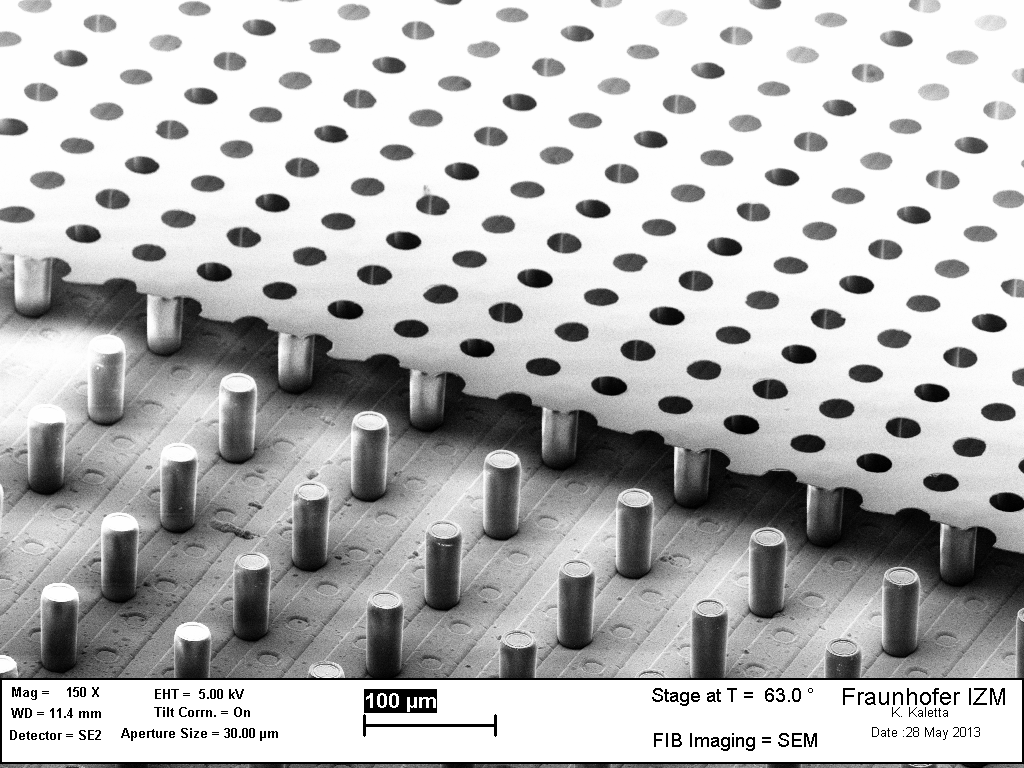
\includegraphics[width=\textwidth]{Tracker/TPC/GridPixes}
		\caption{GridPix detector with a partially removed grid}
		\label{fig:TPC:GridPix:GridPix}
	\end{minipage}
	\hfill
	\begin{minipage}{.49\textwidth}
		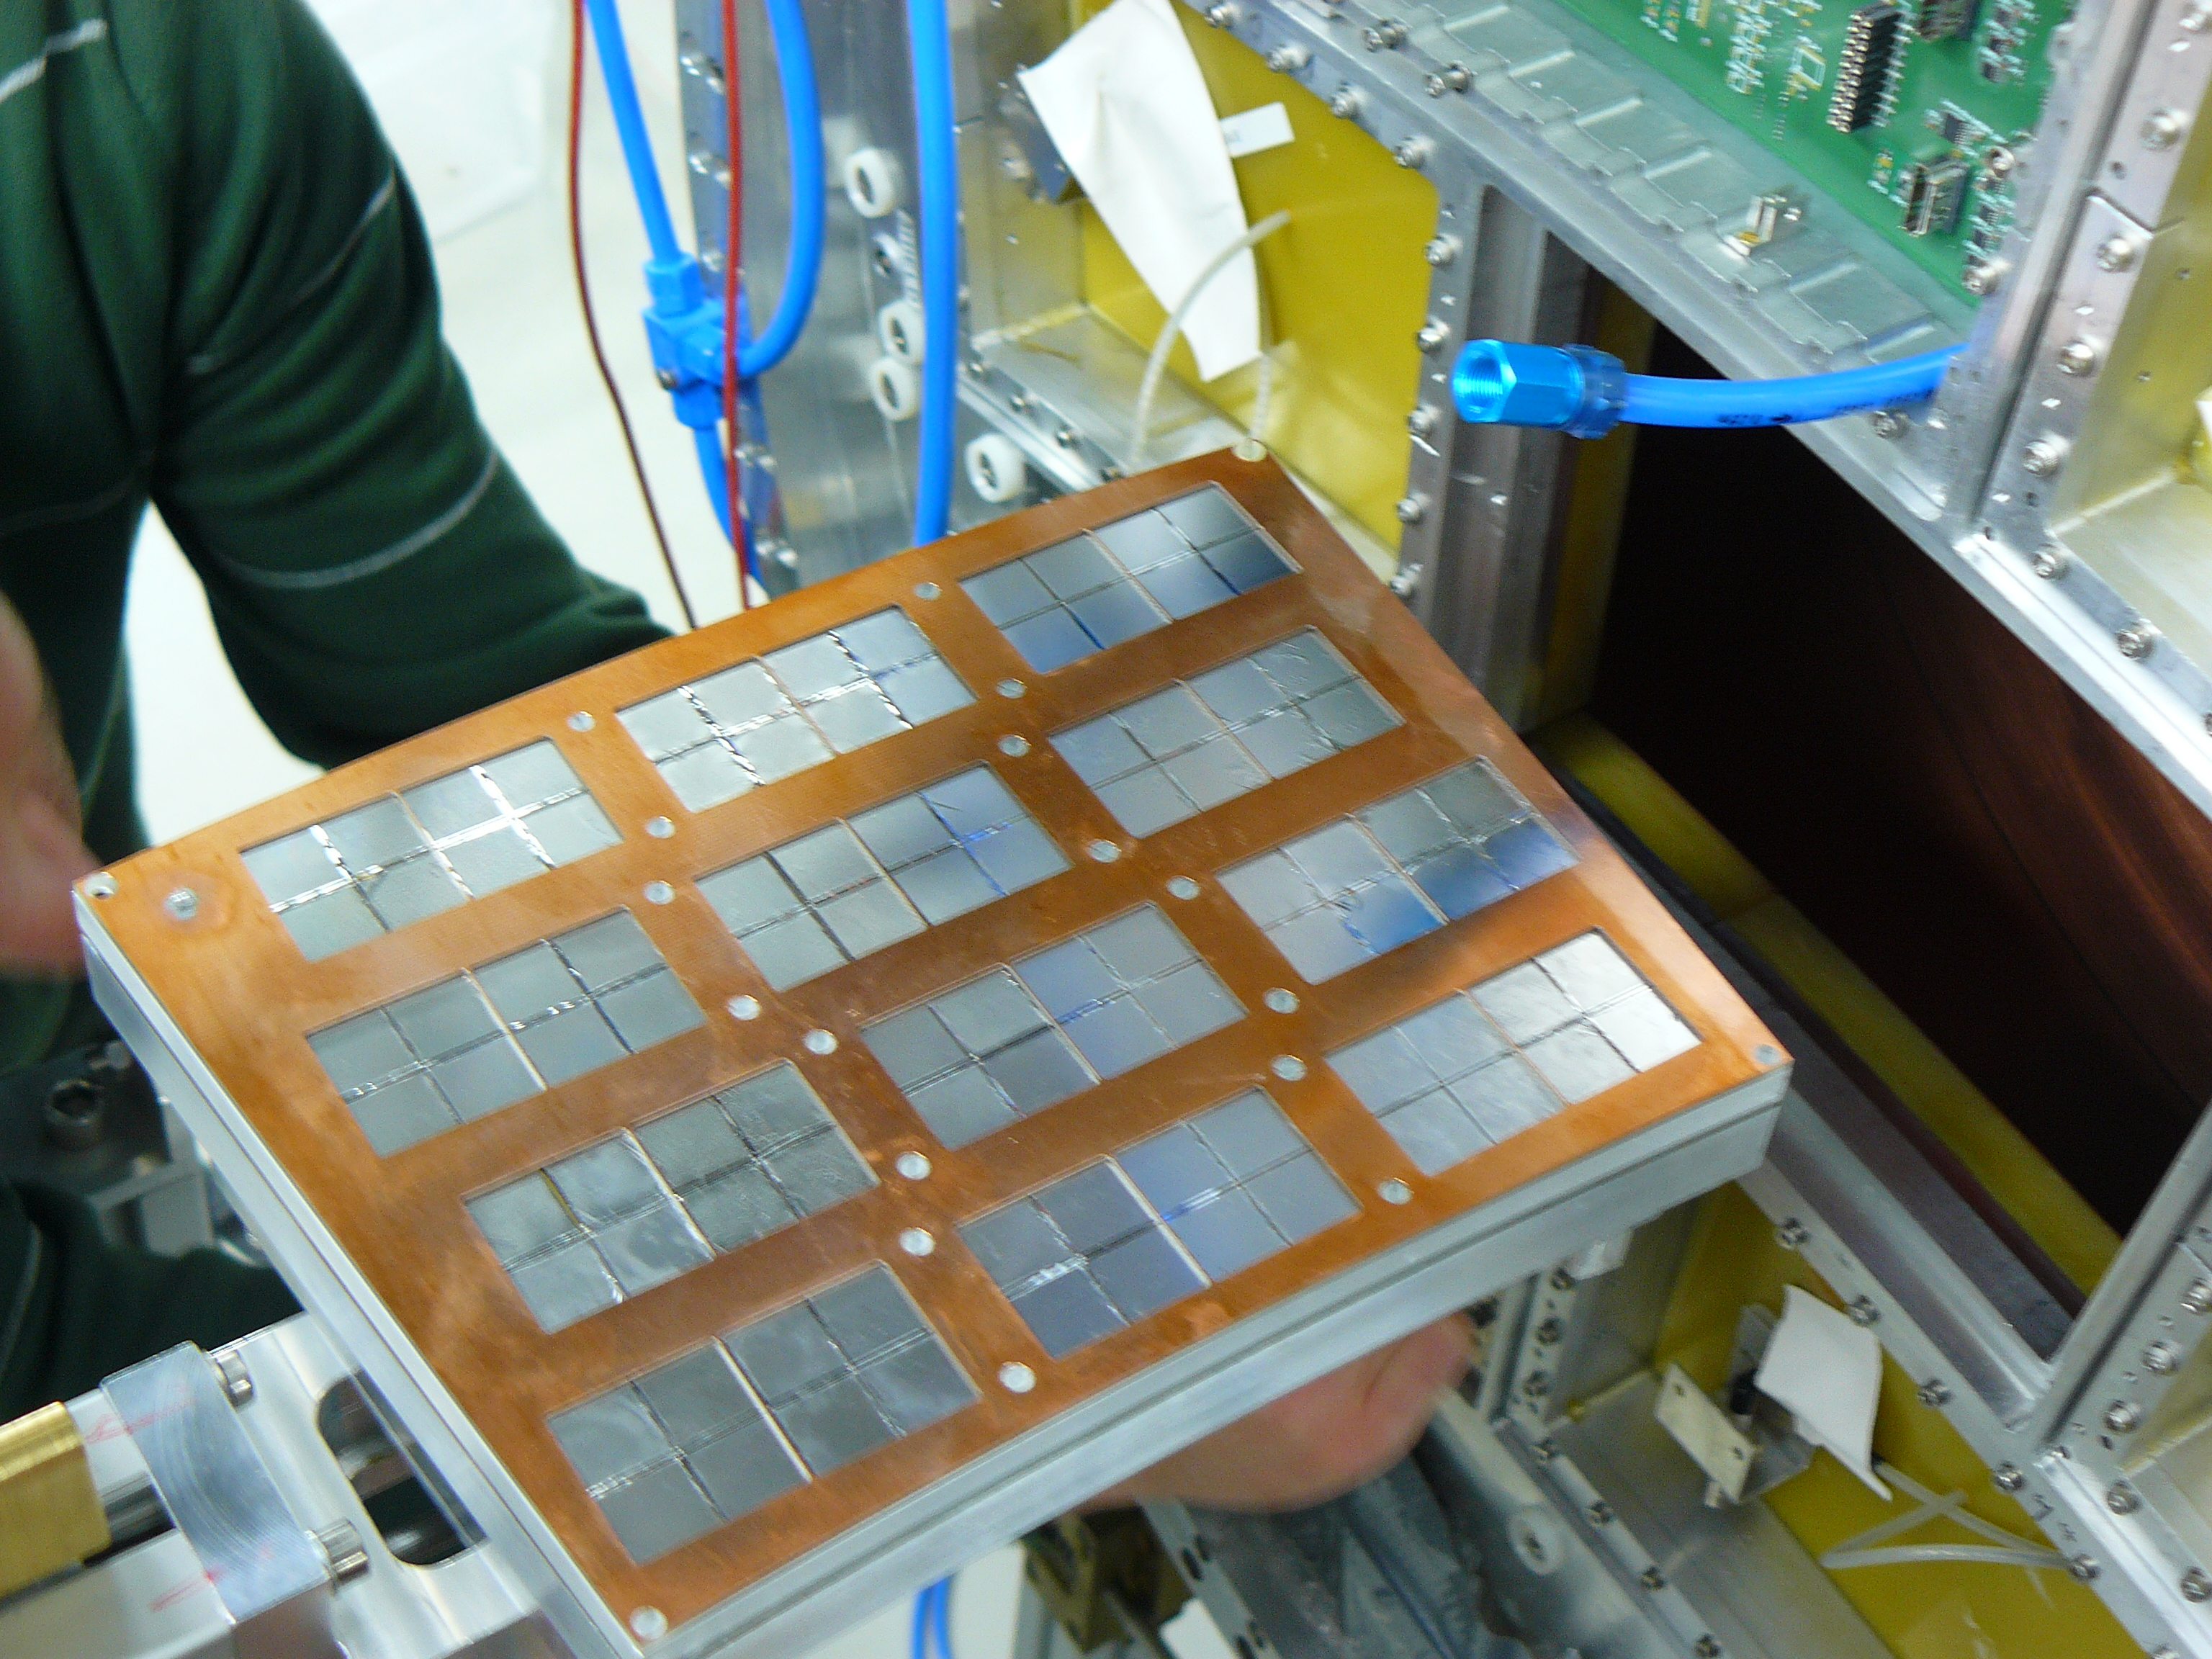
\includegraphics[width=\textwidth]{Tracker/TPC/FullModule}
		\caption{Fully equipped module as it is being mounted}
		\label{fig:TPC:GridPix:module}
	\end{minipage}
\end{figure}

\subsection{Engineering Challenges}
The production of a module with 160 GridPixes requires 4 main components:
\begin{enumerate}
	\item The production of a large number of GridPixes with sufficiently good quality. This has been addressed by the new production method, which is based on complete wafers. The process was developed in collaboration wit the Fraunhofer institute IZM a Berlin and yields up to 400 GridPixes per batch. Figure~\ref{fig:TPC:GridPix:GridPix} shows a GridPix detector with a partially removed grid.
	\item The challenge of the readout is being addressed by the new readout system as described above.
	\item The distribution of the LV power to all ASICs which can reach peek values of \SI{85}{A} at \SI{2.2}{V} was studied in a Master thesis.
	\item Cooling of the ASICs was done by cold water.
\end{enumerate}


\subsection{Future Plans}
Currently, the main focus is on the analysis of the test beam data. The challenge of finding and fitting tracks with several thousand hits is quite different from the standard pad-based TPC analysis. On a longer term all participating institutes are working on software to simulate, reconstruct and analyze data of the ILD-TPC (i.e. about 10,000 hits per track) so that the difference in performance between a pad and a pixel-based TPC can be studied.
On the hardware side we are interested in replacing the Timepix ASIC by the Timepix3 ASIC and produce GridPix detectors with this improved chip, which promises a much better performance, since it is multi-hit capable, can record both time and charge of a each signal and has a much faster digitization frequency. There are also some ideas of how to improve the grid structure and make it more reliable.

\section{Ion Backflow and Gating}
\label{chap:TPC_sec:gating}
Most recent update: 2016-03-28 \\
Contact person: Akira Sugiyama (email: sugiyama@cc.saga-u.ac.jp)\\

\subsection{Introduction}

The distortion of particle tracks due to the accumulation of positive ions in the drift space is the well-known
issue for TPCs, whereby the ions are generated in the gas amplification region and drift back into the TPC drift volume.
Although this ion back flow is much suppressed for the MPGD technology, compared to the earlier MWPC TPCs, it can
still cause significant distortion of tracks when the particle density is high.

Because of the bunch-train structure of the ILC beams (i.e., a  train of ca. 1300 to 2600 bunches during
about \SI{1}{ms}
and a train-repetition rate of \SI{5}{Hz}), the ions flow back from the gas amplification and will form a few discs
of about \SI{1}{cm} thickness in the TPC drift volume where they slowly drift toward the TPC central cathode.
There will be three such ion discs during one train of normal ILC operation, and each disk will modify the trajectory
of the drifting electrons, resulting in the distortion of tracks. The simulations of this distortion at ILC
were made by several people, details can be found in \cite{LC-DET-2012-079,Fujii_IonEffects}.
Figure~\ref{Fig1gating} shows the azimuthal displacement of drift electrons by the ion
disks for different radial positions of TPC with three ion disks in the drift space at the drift distances
indicated by the red lines.

\begin{figure}
\centering
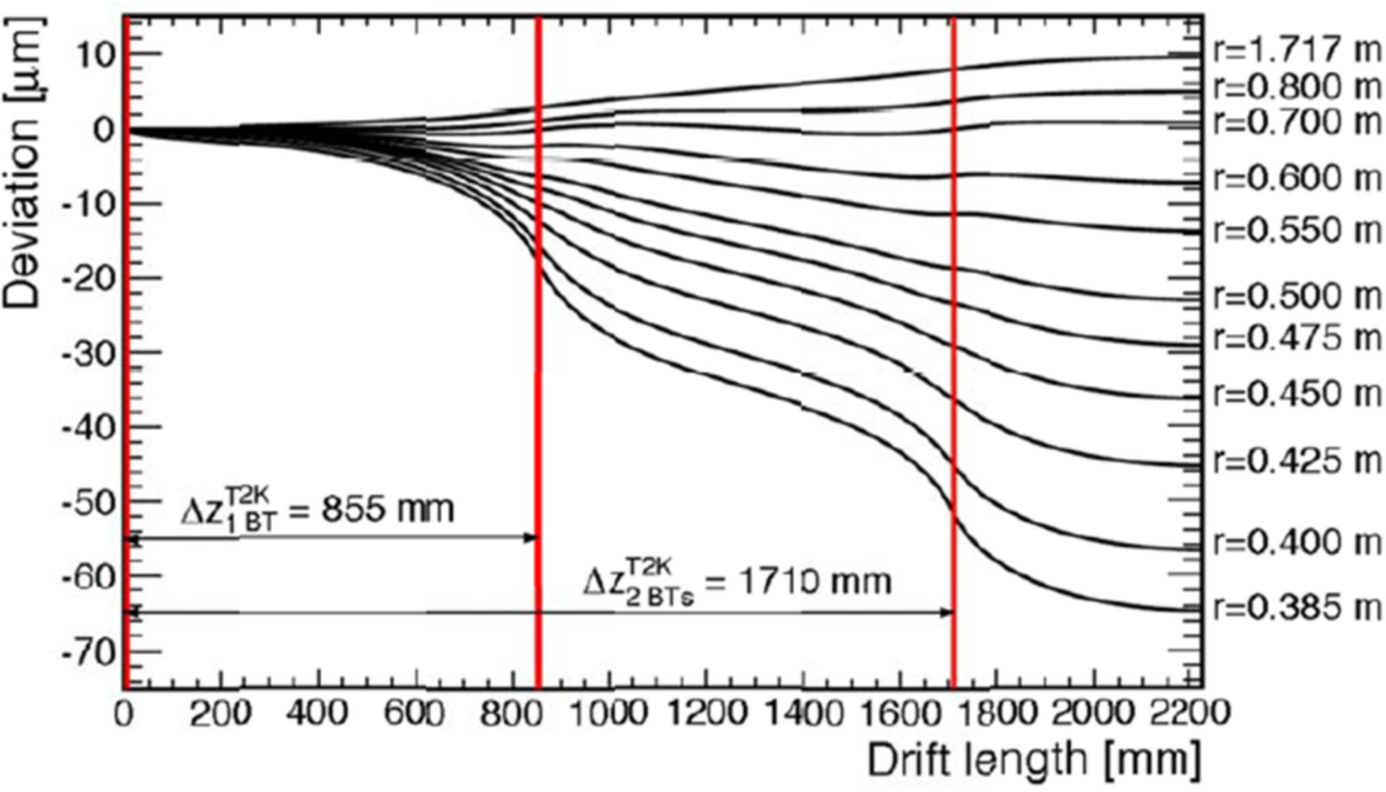
\includegraphics[width=.7\textwidth]{Tracker/TPC_Bonn/plots/TPC-Gate_Fig1gating.pdf}%
\caption{\label{Fig1gating} {Displacement due to the positive-ion discs.}}
\end{figure}

In  Fig.~\ref{Fig1gating} it is assumed that for every drift electron one positive ion drifts back.
The actual amount of displacement should therefore be multiplied by the ratio of the gas amplification
factor to the suppression factor of the ion backflow of the MPGD system. Since the suppression factor by the
MPGD system has been measured to be in the order of order 10$^{-3}$ at
best \cite{Fujii_IonEffects}, the ratio will be larger than one for a gas gain of a few thousand, and distortions larger
than \SI{60}{\micro m} in some parts of TPC would be expected.

At the ILC a TPC point resolution of \SI{100}{\micro m} or better is required by the physics. Thus it is
necessary to either install an efficient gating device to block the ions from the gas amplification, or to correct
the track distortion. Because the machine backgrounds at ILC may not be stable enough to make a reliable
correction possible, an efficient gating device will be needed. Fortunately the bunch-train configuration of ILC
has an ideal time structure for ion gating. The positive ions drift back around \SI{5}{mm} during
the \SI{1}{ms} bunch-crossing period, and can be absorbed by the ion gate which is `closed' (explanation
below) during next \SI{200}{ms} between the bunch trains.

For the expected particle density at ILC, the track distortion by the
{\em{primary}} ions produced in the LCTPC volume is small and has negligible effect.

\subsection{Engineering Challenges: a Wire Gate or a GEM Gate}

Ion gates used for TPCs in past collider experiments consisted of a wire grid. The operation and
structure of the wire gate is well known and can be used for the LCTPC. Figure~\ref{Fig2gating} shows
a simple mechanical prototype of such a wire gate mounted on an Asian GEM module.

\begin{figure}
\begin{center}
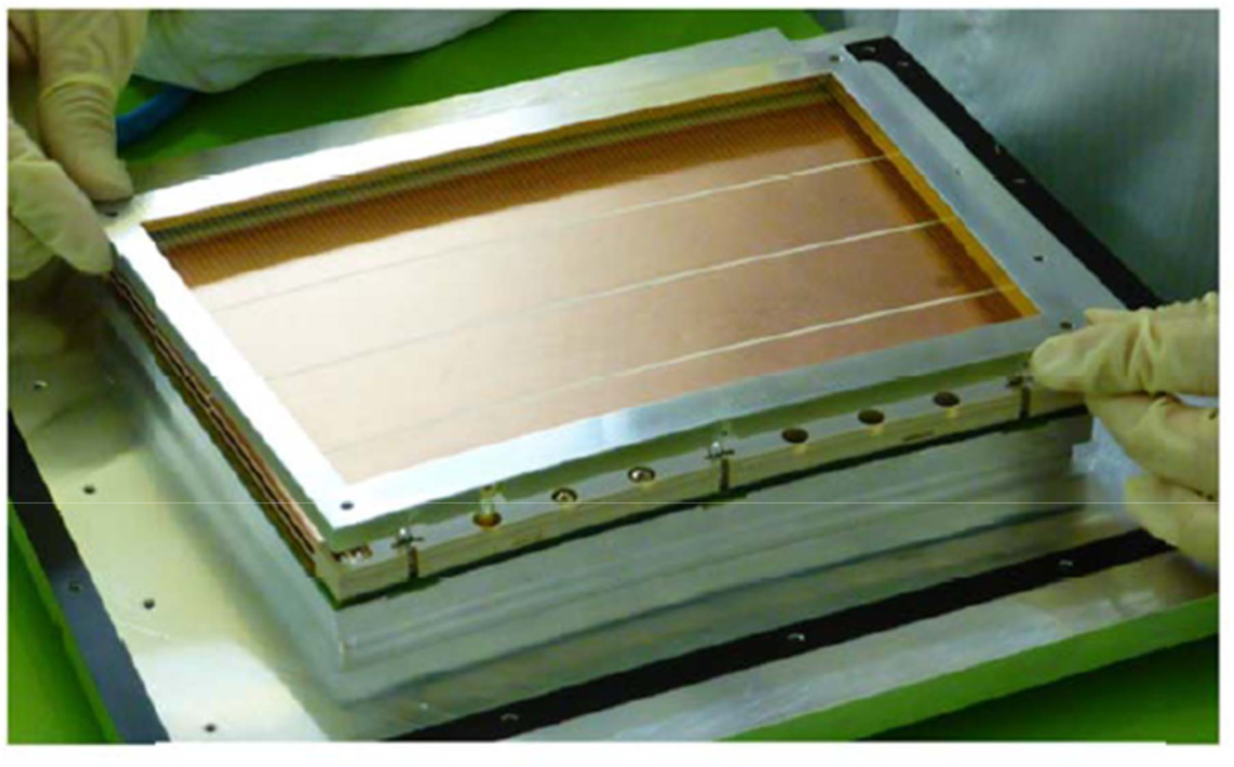
\includegraphics[width=.7\textwidth]{Tracker/TPC_Bonn/plots/TPC-Gate_Fig2gating.pdf}%
\caption{\label{Fig2gating} {Prototype wire gate installed on the Asian GEM module.}}
\end{center}
\end{figure}

The disadvantage of a wire gate for the LCTPC module is to deteriorate the advantages of an MPGD TPC:
the material and space budgets are increased because of the mechanical structure needed to support the many
stretched wires on the module. Therefore, the wire gate is kept as a backup option for the LCTPC, and efforts
are focused on the development of the gate using a GEM foil.

The idea of the GEM gate was proposed by F.~Sauli in 2006 \cite{Sauli2006269}.
The ions from the gas amplification have to be absorbed by the electrode of the gate-GEM in the gate-closed condition.
`Closed' is where the electric field across the gate-GEM is reversed by changing the potential of the bottom
electrode of the gate by about \SI{10}{V}. In the gate-open condition the drift electrons need to reach
to the gas amplification region with a high efficiency in order to not deteriorate the LCTPC resolution
due to loss of signal.

Details of the simulation of GEM gate using the Garfield++ may be found in \cite{LC-DET-2012-079}. Experience was that it is easy
to stop the ions with the necessary suppression factor of 10$^{-4}$ or smaller. On the other hand, it is more
of a challenge to keep a very high efficiency of the drift electrons passing through the gate-GEM in the gate-open
condition. This is because the efficiency is limited by the optical transparency of the gate-GEM when a TPC
is used in a high magnetic field (as in the \SI{3.5}{T} field of ILD) and with a high-$\omega\tau$ gas mixture,
such as the T2K gas \cite{Behnke:2013lya,ref4T2Kgas_ishikawa,Kobayashi201137,Kobayashi2013122} foreseen for the LCTPC. In this condition the drift electron tends to follow the
magnetic field lines rather than the electric field lines, which makes the optical transparency an important parameter .

The first GEM gate prototype for the Asian GEM module for the TPC large prototype (LP) beam test at
DESY in 2009 was \SI{14}{\micro m} thick with the round GEM holes of
\SI{90}{\micro m} diameter and \SI{140}{\micro m} pitch. It had a maximum electron
transmission of 50\% in the magnetic fields of \SI{1}{T} and \SI{0}{T}. It was clear that a GEM
with bigger holes and a narrow rim was needed, that is with larger optical transparency. Simulations found that
GEM holes of the honeycomb shape with very thin rims would maximize the optical transparency.

\begin{figure}
\begin{center}
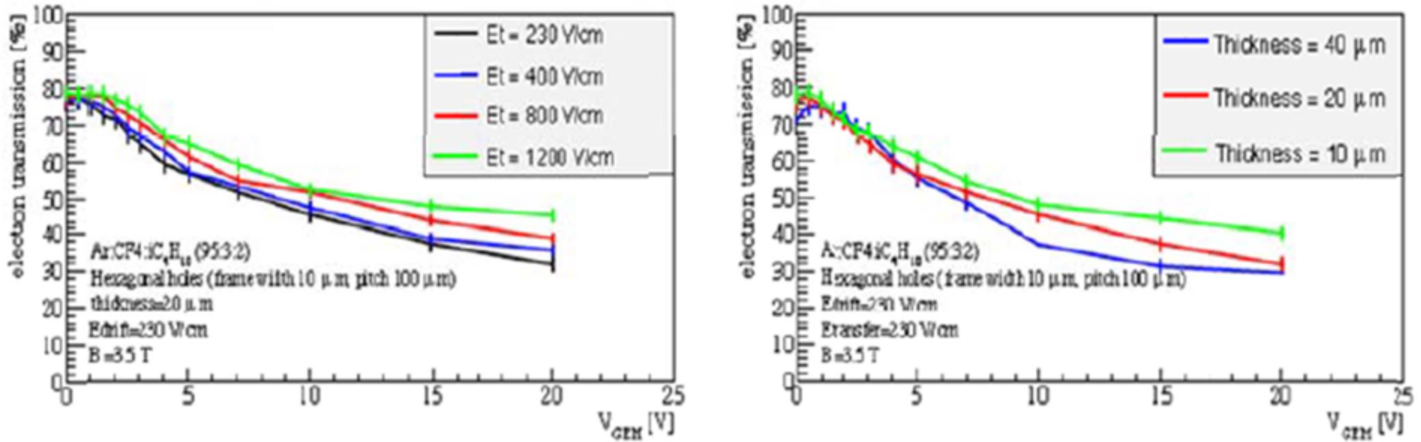
\includegraphics[width=.7\textwidth]{Tracker/TPC_Bonn/plots/TPC-Gate_Fig3gating.pdf}%
\caption{\label{Fig3gating} {The electron transmission simulated for a gate-GEM with the honeycomb-shaped holes of pitch \SI{100}{\micro m} and rim width \SI{10}{\micro m}.}}
\end{center}
\end{figure}

As is seen the simulation results shown in Fig.~\ref{Fig3gating}, the thin gate GEM with
honey\-comb-shaped holes of \SI{100}{\micro m} pitch and \SI{10}{\micro m} rim width is shown to reach
an electron transmission of 80\%. However, a rim width of \SI{10}{\micro m} turns out to be very difficult to produce;
an alternative is presented in the next subsection.

\subsection{Recent Milestones}

In 2013 the Japanese LCTPC group started the actual fabrication of the GEM gate with the large
optical transmission. With the limitations of the available processes of GEM, the specifications
were set using  Fig.~\ref{Fig45gating}(lower)
which are summarized in the Table 1. The target is to fabricate a gate GEM with  honeycomb shape holes
of around \SI{300}{\micro m} diameter and  rim-width of \SI{35}{\micro m} or smaller. The immediate goal
of this study is to test the Asian LP module with this GEM gate in the DESY test beam in 2016.

\begin{table}
\begin{center}
\begin{tabular}{|l|l|}
\hline
Item & Specification \\%$\sim$
\hline
\hline
Optical aperture ratio &  80\% \\
Hole size       & \SI{300}{\micro m}\\
Hole pitch       & \SI{335}{\micro m}\\
Rim size            & \SI{35}{\micro m}  \\
Insulator thickness  & \SI{25}{\micro m}\\
Foil size            & $170\times\SI{220}{mm}$ \\
\hline
\end{tabular}
\caption{\label{gatespecs} Specification of the gate-GEM in the current study.}
\end{center}
\end{table}

Prior to the fabrication of a large, module-sized gate, many small samples of
\SI{10}{cm} $\times$ \SI{10}{cm} were produced to test different processing techniques.
Although some samples by the standard single-mask chemical process were promising, limited resources required that
a major effort be continued with Fujikura Ltd.~\cite{ref5fujikuraltd} using their laser-chemical hybrid technology to produce
FPCs (flexible printed circuits). Details of the Fujikura process for the gate-GEM were presented at MPGD2015 \cite{MPGD2015_gate}.
Figure~\ref{Fig45gating}(upper) shows the structure of one of the gate-GEM small samples made by Fujikura
according to the specifications in Table \ref{gatespecs}.

\begin{figure}
\begin{center}
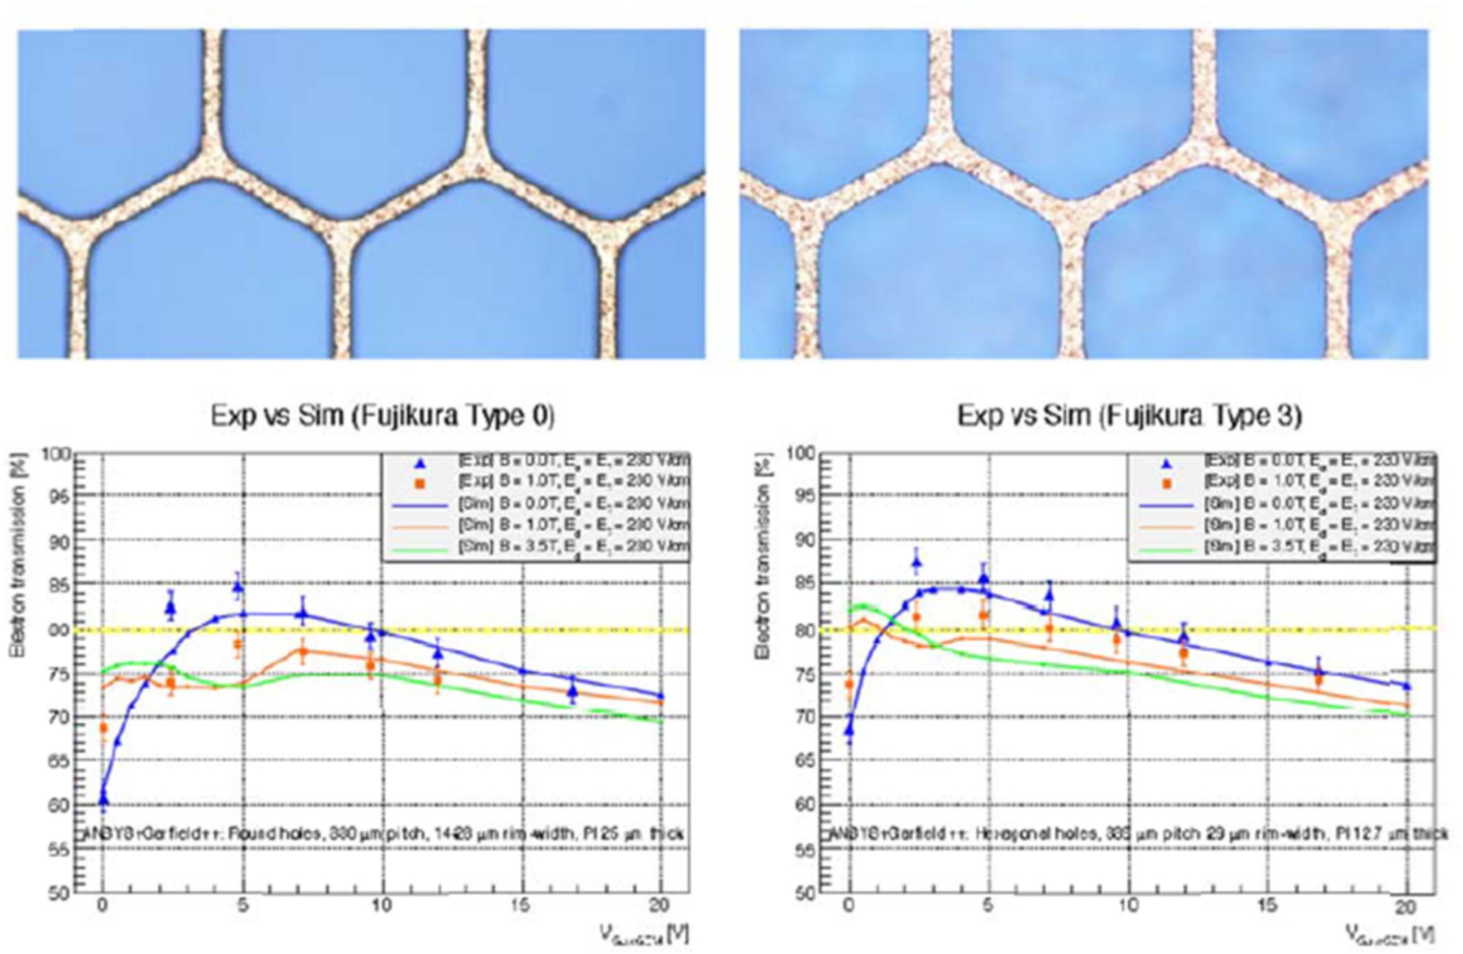
\includegraphics[width=.7\textwidth]{Tracker/TPC_Bonn/plots/TPC-Gate_Fig45gating.pdf}%
\caption{\label{Fig45gating} {Upper: Honeycomb hole structure of the gate-GEM.
The pitch of the holes is \SI{335}{\micro m}, the rim width \SI{29}{\micro m}.
The polyimide insulator is \SI{12.7}{\micro m} thick.
Lower: Preliminary results of the electron transmission measurement are compared to simulation
as functions of the GEM voltage for two types of gate-GEMs. In the left panel are
results for gate-GEM with round holes; in the right panel results for the gate-GEM with the honeycomb-shaped holes.}}
\end{center}
\end{figure}

The electron transmission was measured for these samples, and
Fig.~\ref{Fig45gating}(lower) shows the results of the measurement compared to the simulation in magnetic fields
of 0, 1 and \SI{3.5}{T}. In the left panel, the results for the sample with round holes, and in the right panel
for the sample with honeycomb-shaped holes.  The electron transmissions at 0 and \SI{1}{T} were confirmed
to be better than 80\% while the optical transmission was calculated to be 82\% for the honeycomb-shaped-hole sample.

Having established the best configuration and the best process for the gate GEM with the small samples,
the focus has now moved to the fabrication of the gate-GEM with  the size of the Asian GEM module (Fig.~\ref{Fig6gating}).
Here the major issue for the fabrication is to minimize any defects in the electrode circuit of the gate-GEM
so that there is 100\% stopping power of the ions.

\begin{figure}
\begin{center}
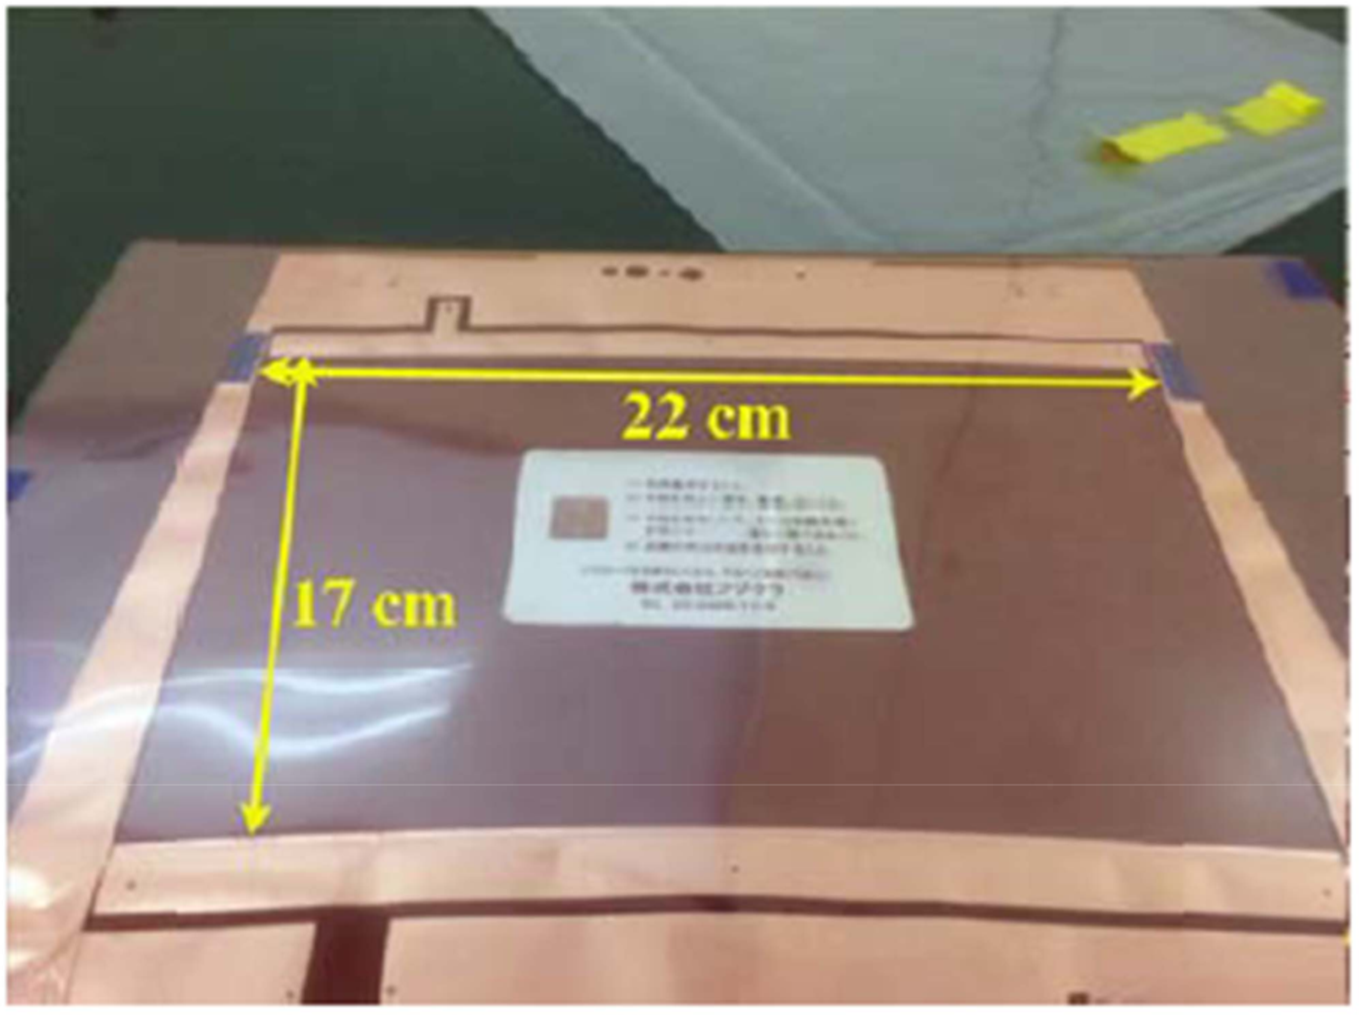
\includegraphics[width=.7\textwidth]{Tracker/TPC_Bonn/plots/TPC-Gate_Fig6gating.pdf}%
\caption{\label{Fig6gating} {A sample gate-GEM for the Asian module.}}
\end{center}
\end{figure}

\begin{figure}
\begin{center}
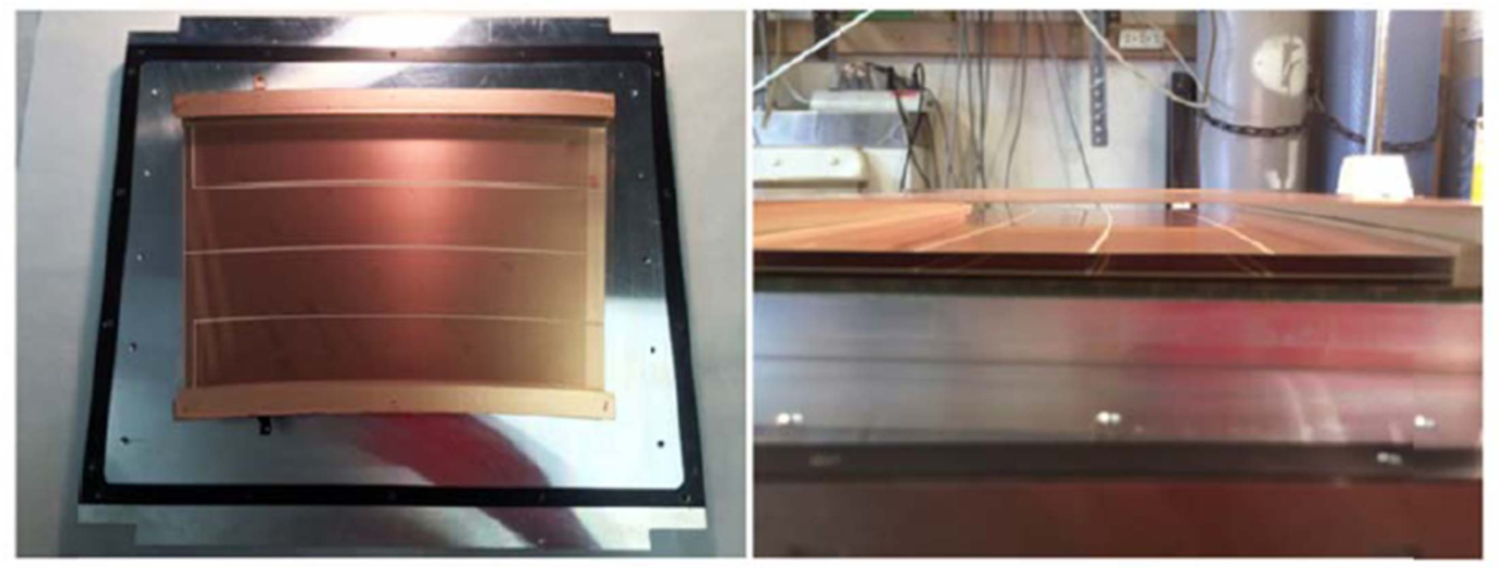
\includegraphics[width=.7\textwidth]{Tracker/TPC_Bonn/plots/TPC-Gate_Fig78gating.pdf}%
\caption{\label{Fig78gating} {Left panel: Test mounting of the gate-GEM. Right panel: Test assembly of the gate GEM on the Asian GEM module.}}
\end{center}
\end{figure}

Figure~\ref{Fig78gating}(left) shows the test mounting of the gate-GEM on the module. As can be seen,
the pattern of the amplifier GEM below the thin gate-GEM can be seen clearly, indicating a  high optical transparency.
Figure~\ref{Fig78gating}(right) is a picture of a test assembly of the gate-GEM on the module.

\subsection{Future Plans}

The production process for the large gate-GEM has been essentially established,
and a few of the good samples for the Asian GEM module have been delivered for testing.
The preparations for measuring the electron transmission by using a laser beam are under way.
Although the Asian model is designed to have a GEM gate mounted on it,
there may be more issues coming up, and some optimization of the mounting method and the module structure
might become necessary for the design of the LCTPC. Beside some difficulties to stretch such a thin
GEM stably, some consideration on the possible ion leak through the module boundaries
for the Asian GEM modules may be needed.

\section{Electronics, DAQ and Cooling}
\label{chap:TPC_sec:electronics}
Most recent update: 2020-05-12 \\
Contact person: Leif J{\"o}nsson (email: leif.jonsson@hep.lu.se)

\subsection{Introduction}
The readout electronics for the TPC has to be adapted to the design of the tracking chamber and the beam structure of the collider. The physics goals of the ILC requires high momentum resolution and two-track separation, which drive the track reconstruction in the $r\text{-}\varphi$-plane to pad sizes of small dimensions. For the $r\text{-}z$-plane a short shaping time and a high sampling rate is necessary to provide the best possible timing information. However, at the same time the noise level has to be kept at a manageable level. The sampling depth has to match the sampling frequency in order to cover the full drift length. The front end electronics has to be accommodated within pad modules, with a channel occupancy that is smaller than the pad size to allow space for the mounting frame, the voltage supply and the cooling system.

The power consumption of the front-end electronics should be kept low such that the heat dissipation does not lead to a temperature increase in the TPC-gas of more than typically \SI{1}{\degreeCelsius} after cooling. In this respect, power pulsing, where the front-end electronics is switched off for about \SI{199}{ms} between the bunch trains, helps significantly.

The readout electronics presently under development aims to demonstrate that the channel occupancy can be made compatible with the small pad size foreseen. It is based on the CERN SALTRO16-chip (shown in Figure~\ref{fig:TPC:SaltroPic}), which integrates the analogue and digital signal processing of the incoming signals within the same compact circuit. Feasibility studies of the readout concept has to be performed with existing ASICs. This prototype system is described below. A final dedicated ASIC for the ILD TPC will have a much larger channel density and higher degree of integration of functionalities and will thus occupy less space than the present prototype electronics. The size of the die is $8.7 \times \SI{6.2}{mm^2}$ and it contains 16 readout channels. The chip is programmable with respect to gain, rise time, decay time and polarity. The sampling can be clocked at frequencies 5, 10, 20 and \SI{40}{MHz} and it allows for power pulsing.

\begin{figure}
    \centering
    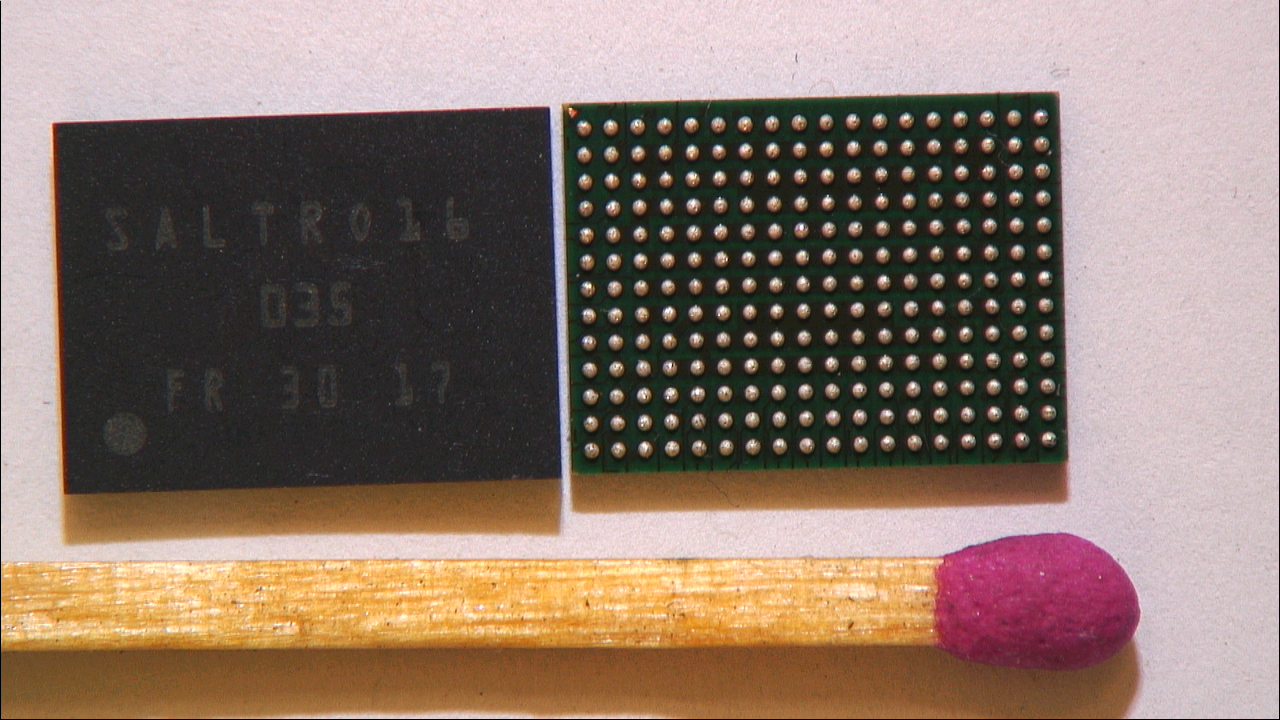
\includegraphics[width=.5\linewidth]{Tracker/TPC_Bonn/plots/TPC-Electronics_JonssonsALTRO_Chip-Photo_07062018}
    \caption{Photograph of two SALTRO-16 chip side-by-side and a matchstick for comparison.}
    \label{fig:TPC:SaltroPic}
\end{figure}

In total 840 untested dies have been obtained and delivered to the company, which performs the packaging into small capsules of size $12\times\SI{9}{mm^2}$. The bottom side of the chip contains small tin balls organized in a BGA pattern for soldering of the packaged SALTRO16 chip on so-called Multi-Chip Modules (MCM).

Eight SALTRO16 chips are mounted on an MCM, which also contains a CPLD (Complex Programmable Logic Device) controlling the data flow. The MCM-board is the smallest unit in the front end electronics and it is attached to the pad plane via four micro-connectors, whereas on the opposite side of the board there are two connectors, via which the low voltage is distributed and the signals are transmitted. The MCM-board is designed in High Density Interconnect (HDI) technology, by which the number of layers is significantly reduced compared to conventional PCB design. The dimensions of the MCM-board are $32.5 \times \SI{25}{mm^2}$ and serves 128 readout channels. This corresponds to a channel occupancy of about $\SI{6.4}{mm^{2}}$, although some space is also required for the high voltage connectors of the gas amplification system (GEMs and Micromegas) and the cooling system.

A serial readout system is used for the signal transfer to the DAQ computer. The MCM-board and the Scalable Readout Unit~\cite{1748-0221-8-03-C03015} (SRU) communicate directly via the Data Trigger Control (DTC) link. Communication, data transfer and control, between the SRU and a DAQ computer is done via Ethernet.

Cooling of the front end electronics is a challenge since the size of the cooling system must match the smallness of the electronics and still provide efficient cooling. The total power consumption of an MCM-board in continuous operation
is \SI{3203}{mW} on the top side and \SI{3028}{mW} on the bottom side. In power pulsing mode, with a bunch train of \SI{725}{\micro \second}, containing 1312 bunches, the power dissipation is reduced to about \SI{223}{mW} per MCM-board on the top side and \SI{48}{mW} on the bottom side. A cooling system with cooling pipes that run on top of the MCM-boards, using two-phase \ce{CO2} coolant, is considered. Another possibility would be to use micro-channel cooling, which has been developed by the semiconductor community. Such systems are presently further developed within the AIDA2020 project, for applications in high energy physics experiments. The ILC cycle is not realistic in a test beam environment as at e.g. DESY. To get a reasonable trigger rate is e.g. a cycle with \SI{5}{ms} beam at \SI{10}{Hz} more useful, which corresponds to \SI{343}{mW} per MCM-board on the top side and \SI{168}{mW} on the bottom side, in power pulsing mode.

\subsection{Recent Milestones}
A system for testing the SALTRO-16 chips has been built and debugged. We are aiming at a readout system with at least 10,000 channels, which requires a yield of about 75\%. The tests of two pre-series have been completed. The first one, containing 34 chips, gave a lower yield, requiring an improved bonding procedure. The second pre-series, containing 55 chips, gave a yield well above the goal and we decided to go ahead with the full production.
The delivery of the bulk of the chips happened at the end of the year 2018.
The design of the final 16-layer MCM-board was completed and the boards were manufactured. By pushing the boundaries of commercially available assembly techniques to the limit, read-out of sensor pads, as small as \SI{6.3}{\milli\meter\squared}, could be achieved with the MCM-board connected parallel to the pad plane. We have simplified the design by reducing the number of separate voltage levels needed from seven to two. Initial tests revealed some bugs in the PCB design, most of which could be fixed. Prior to the performance tests of the MCM-board, a prototype LV board, providing low voltage supply for a single MCM-board, was designed and produced. The design of the final LV-board intended for five MCM-boards is well under way.
For tests of the performance, two MCM-boards were mounted by the DESY electronics group at the end of 2019. The tests showed that data could be read and written and thus the concept was proven to work. Pedestal runs were performed and gave good results, and the noise performance was promising. However, this first prototype of the readout board required some corrections, which have been implemented and the next version of the MCM PCB has been ordered. The official delivery time was 8.5.2020, but at the time of writing the supplier claims a delay of about one week. The assembly by the DESY electronics group will follow together with further tests.

\subsection{Engineering Challenges}
The final aim is to produce front end electronics, high voltage supply and a cooling system which are compatible with a pad size of $1 \times \SI{6}{\milli\meter\squared}$. The compactness of the electronics and the space limitations are major challenges, as well as designing a suitable and efficient cooling system. An elegant solution for the low voltage supply has to be found and due to space limitations the design of the mechanical support for the electronics is also a challenge.

\subsection{Future Plans}
In case the upcoming tests are successful, a fully mounted MCM-board will be produced and tested.
Until we have got help with the FPGA-programing we will not be able to test the rest of the chips and
thus no further MCM-boards can be produced.
The design of the micro-channel cooling support structure is ready and production is planned.

\section{Mechanics and Calibration}\label{chap:TPC_sec:mechanics}
Most recent update: 2016-03-28\\
Contact person: Ties Behnke (email: ties.behnke@desy.de)\\

\subsection{Introduction}
A key component of the TPC at a future collider will be the design and construction of the field cage. The cage should be light weight, yet mechanically and electrically stable. It should provide support for the cathode and the anode systems, and allow excellent field shaping in between.
To test the concept for such a field cage a prototype has been built as part of the LCTPC test infrastructure \cite{1748-0221-5-10-P10011}. The field cage is made from a light weight composite sandwich structure. The mechanical structure is given by a honeycomb layer, which is covered on the inside and the outside by a glass fibre reinforced epoxy layer. On the inside a Kapton foil provides electrical insulation, and field shaping through a system of copper ring electrodes. On the outside a thin aluminum layer provides grounding. Integrated into the field cage a laser based calibration system is foreseen.

The prototype field cage has been constructed in 2008 and has been used with all different readout technologies since. It is equipped with an aluminum based endplate, which can host up to seven identical readout modules. It is designed to fit into the PCMAG magnet \cite{Yamamoto199475} infrastructure, which is installed at the DESY test beam facility \cite{DESY2TB}.

%Another challenge is the development of a compact and efficient cooling strategy. Currently, CO$_2$ based systems are favoured and are being prototyped.

A large system like the TPC poses particular challenges to calibrate the system and to maintain the calibration. Currently several systems are under consideration.

An important part of the calibration will be done based on data recorded, without special hardware. Tracks will be used to align the different modules relative to each other, and to measure and correct field distortions.

While tracks are an excellent method to derive relative corrections, and to equalise the response, it might be difficult to reach the ultimate absolute resolution without an external unbiased reference. This reference can come from different sources. Within the ILD detector design silicon detectors are foreseen before and after the TPC, which will provide an external reference. These systems can be used to calibrate the field distortions, and to set the scale for the momentum measurement. Another system will be based on laser beams. Laser beams will be used in two ways. Well focused small cross section beams can be inserted into the drift volume, and serve as fake tracks. The ionization along the laser beams is recorded as for normal tracks, and can be used to calibrate the response of the TPC. A wide laser beam can be used to illuminate the cathode of the TPC. Dots or lines of a low work-function material like e.g.~aluminium on the surface of the cathode would then provide well defined spots where the laser
light can liberate electrons. These electrons then drift towards the anode and sample any inhomogeneities on their way. Thus, they can be used to monitor and ---to some extent--- determine the field properties inside the drift volume. Both types of laser beams need to be inserted into the TPC, and will require the design and implementation of sophisticated hardware.

% %\subsection{Recent Milestones}
\subsubsection{Engineering Challenges}
The current field cage has been successfully used in numerous test beam campaigns. However, it has failed to deliver the ultimate mechanical precision which is needed for the demonstration of the anticipated momentum resolution of the TPC system. In particular, the manufacturer has failed to deliver the needed alignment between the anode and the cathode, and has introduced a small overall skew into the field cage. The main challenge will be to develop and build a second generation field cage which fulfills the precision requirements. For this an entirely new tooling is being developed, which should help to ensure the mechanical precision.

The results from this prototype field cage will then be applied to a study of the design of the full field cage for the ILD TPC. A central and so far unsolved engineering challenge is the support of the TPC in the overall detector. Here a combination of light weight, space saving support structures combined with superb mechanical stiffness need to be found. Particular attention will also need to be payed to the behaviour of the system in case of earth quakes, given that the proposed site of the ILC in Japan is located in an earth-quake prone region.

An open and as yet unsolved issue is the design of the central cathode of the TPC. This system is located in the centre of the detector, very difficult to access. It needs to be light weight, yet dimensionally very stable. It will be supplied with high voltage of close to \SI{100}{kV}. The supply of this very high potential in a safe and reliable way is under study and represents significant challenges.

As described above laser beams will be used to calibrate the system. The insertion and guidance of these laser beams present significant challenges. Ways will need to be found to bring the laser beams to the TPC. The laser will have to be installed on the outside of the detector, so that transport ways of several meters through a very crowded environment are needed.

\subsection{Future Plans}
Over the next few years a full engineering design of the ILD TPC will be developed. This will include a detailed simulation of the TPC system, and its mechanical properties, and its integration into the ILD detector as a whole.

Detailed problems which will need to be addressed are:

\begin{itemize}
\item Finite Element Method (FEM) calculations of the field cage and the endplate
\item Optimisation and final decision on the layout of the endplate: size of modules, number of modules, etc.
\item Design of the support system of the TPC in the ILD detector
\item Study of the mechanical properties of the TPC support in view of vibrations and overall stability
\item Design and implementation of a system of laser beams in the TPC drift volume
\item Design and implementation of a system to illuminate the TPC cathode with a laser beam.
\end{itemize}

%Contributing : DESY, KEK, U Cornell, U Hamburg, CEA Saclay, Nikhef, U Victoria

%\subsection{Recent Milestones}

%The cooling system of the PCMAG has been modified from cooling with liquid helium to a system using a closed helium circuit with external compressors and cold heads installed in the PCMAG. This allows a continuous operation over long time periods of several months and improves the usability and safety of the setup.

%Contributing: AIDA, KEK, DESY

%A two-phase CO$_2$ cooling system (TRACI) has been installed at the test beam area and successfully operated at two test beam periods, so far.

%Contributing: KEK, DESY, Nikhef, CEA Saclay
%
%
%\subsection{Engineering Challenges}
%
%The field cage of the LPTPC has to be mechanically and electrically stable, while keeping the material budget of its wall structure at about 1\% of X$_0$. Its mechanical tolerances are very tight to ensure an electric field homogeneity of $10^{-4}$.
%
%\subsection{Future Plans}
%
%The first field cage of the LPTPC had been designed at DESY and built by an external company.  The allowed mechanical tolerance of max. $0.5\,\mathrm{mm}$ for the tilt of the cylinder axis was not kept. A new field cage will be constructed in-house at DESY. Material tests and the preparation of the required construction tools are ongoing.

